
\documentclass[10pt,xcolor={dvipsnames}]{beamer}
\usetheme[
  ]{Feather}
  
% If you want to change the colors of the various elements in the theme, edit and uncomment the following lines

% Change the bar colors:
\setbeamercolor{Feather}{fg=NavyBlue!20,bg=NavyBlue}

% Change the color of the structural elements:
\setbeamercolor{structure}{fg=NavyBlue}

% Change the frame title text color:
\setbeamercolor{frametitle}{fg=black!5}

% Change the normal text colors:
\setbeamercolor{normal text}{fg=black!75,bg=gray!5}

%% Change the block title colors
\setbeamercolor{block title}{use=Feather,bg=Feather.fg, fg=black!90} 


% Change the logo in the upper right circle:
%\renewcommand{\logofile}{example-grid-100x100pt} 
%% This is an image that comes with the LaTeX installation
% Adjust scale of the logo w.r.t. the circle; default is 0.875
% \renewcommand{\logoscale}{0.55}

% Change the background image on the title and final page.
% It stretches to fill the entire frame!
% \renewcommand{\backgroundfile}{example-grid-100x100pt}

%-------------------------------------------------------
% INCLUDE PACKAGES
%-------------------------------------------------------

\usepackage[utf8]{inputenc}
\usepackage[french]{babel}

\usepackage[T1]{fontenc}
\usepackage{tikz}
% \usepackage{helvet}

%% Load different font packages to use different fonts
%% e.g. using Linux Libertine, Linux Biolinum and Inconsolata
% \usepackage{libertine}
% \usepackage{zi4}

%% e.g. using Carlito and Caladea
\usepackage{carlito}
\usepackage{caladea}
\usepackage{zi4}

%% e.g. using Venturis ADF Serif and Sans
% \usepackage{venturis}

%-------------------------------------------------------
% DEFFINING AND REDEFINING COMMANDS
%-------------------------------------------------------

% colored hyperlinks
\newcommand{\chref}[2]{
  \href{#1}{{\usebeamercolor[bg]{Feather}#2}}
}

%-------------------------------------------------------
% INFORMATION IN THE TITLE PAGE
%-------------------------------------------------------

\title[] % [] is optional - is placed on the bottom of the sidebar on every slide
{ % is placed on the title page
      \textbf{Le Développement Web Responsable}
}



\author[Dorine Tabary]
      {\ttfamily dorine.tabary@univ-fcomte.fr}


\institute[]
{%
      Université de Franche-Comté\\
      Sciences et Techniques
}

\date{\today}

%-------------------------------------------------------
% THE BODY OF THE PRESENTATION
%-------------------------------------------------------

\begin{document}

%-------------------------------------------------------
% THE TITLEPAGE
%-------------------------------------------------------

{\1% % this is the name of the PDF file for the background
\begin{frame}[plain,noframenumbering] % the plain option removes the header from the title page, noframenumbering removes the numbering of this frame only
  \titlepage % call the title page information from above
\end{frame}}


\begin{frame}{Table des matières}{}
\tableofcontents
\end{frame}

\section{Le changement climatique}

\begin{frame}{Le changement climatique}{Le réchauffement et ses conséquences}

\begin{figure}
	\centering
	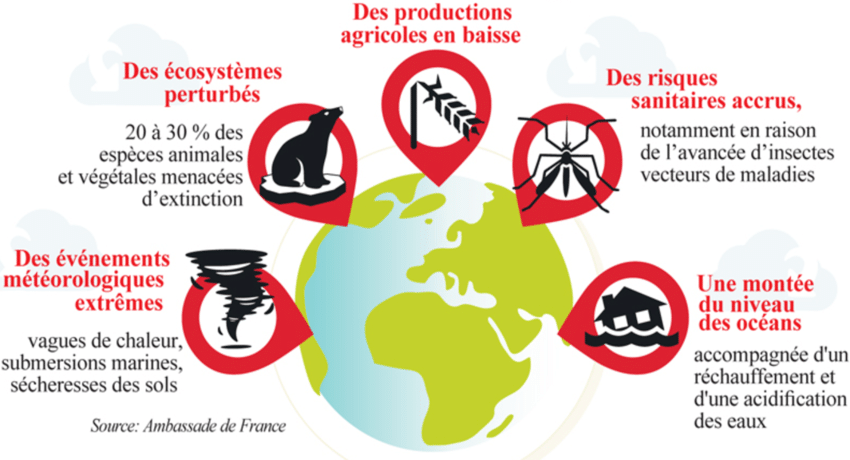
\includegraphics[scale=0.37]{Feathergraphics/effetChgmtClimat.png}
\end{figure}

\end{frame}
\begin{frame}{Pollution liée à l'activité humaine}{et focus sur le numérique}
\begin{figure}[h!]
\begin{minipage}[b]{0.5\linewidth}
\begin{block}{$CO_2$ d'origine humaine}
	\begin{itemize}
		\item Production energétique : $39\%$
		\item Transport : $23\%$			
		\item Industrie : $22\%$		
		\item Résidentiel : $10\%$		
		\item Tertiaire : $4\%$	
		\item Agriculture : $2\%$
	\end{itemize}
\end{block}
	
\end{minipage}\hfill
\begin{minipage}[b]{0.45\linewidth}   
\begin{tikzpicture}
\node[blue] at (1,3)   (a) {Fabrication};
\node[blue] at (3.5, 1.5)   (b) {Utilisation};
\node[blue] at (1, 0)   (c) {Destruction};

\draw[->,>=latex, line width=1mm,color=blue!50] (a) to[bend left=50] (b);
\draw[->,>=latex, line width=1mm,color=blue!50] (b) to[bend left=50] (c.east);
\draw[->,>=latex, line width=1mm,color=blue!50] (c.west) to[bend left=50] (a.west);
\node (ordi) at (1.4,1.5) {
\includegraphics[scale=0.08]{Feathergraphics/ordi.png}};
\end{tikzpicture}


\end{minipage}

\begin{alertblock}{Question}
	Quelle est la part du numérique ?~\cite{ImpactNumerique}~\cite{greenpeace}
\end{alertblock}
\end{figure}

\end{frame}

\begin{frame}{Pollution liée à l'activité humaine}{et focus sur le numérique}
	\begin{figure}[h!]
		\begin{minipage}[b]{0.5\linewidth}
			\begin{block}{Origine humaine}
				\begin{itemize}
					\item \textcolor{blue}{Production energétique : $39\%$}%20pourcent 
					\item Transport : $23\%$			
					\item Industrie : $22\%$		
					\item Résidentiel : $10\%$		
					\item Tertiaire : $4\%$	
					\item Agriculture : $2\%$
				\end{itemize}
			\end{block}
			
		\end{minipage}\hfill
		\begin{minipage}[b]{0.45\linewidth}   
			\begin{tikzpicture}
			\node[blue] at (1,3)   (a) {Fabrication};
			\node[blue] at (3.5, 1.5)   (b) {Utilisation};
			\node[blue] at (1, 0)   (c) {Destruction};
			
			\draw[->,>=latex, line width=1mm,color=blue!50] (a) to[bend left=50] (b);
			\draw[->,>=latex, line width=1mm,color=blue!50] (b) to[bend left=50] (c.east);
			\draw[->,>=latex, line width=1mm,color=blue!50] (c.west) to[bend left=50] (a.west);
			\node[opacity=0.3] (ordi) at (1.4,1.5) {
\includegraphics[scale=0.08]{Feathergraphics/ordi.png}};
			\node (ordi2) at (1.4,1.5) {\Huge \textbf{$4\% \nearrow$} };
			\end{tikzpicture}
			
			
		\end{minipage}
	
	\begin{block}{Pourquoi ?}
	\cite{bachelet2007global}~\cite{webeco}~\cite{shift}	%34 000 000 000 de smartphones, consoles et télés.
	\end{block}
	\end{figure}
	
\end{frame}



\begin{frame}{Impact du numérique}{Origine}
%--	\begin{figure}[h!]

\begin{block}{Fabrication à partir de ressources naturelles}
\begin{figure}[h!]

\begin{minipage}[b]{0.5\linewidth}
Les minerais rares
\begin{itemize}
    \item Bismuth
    \item Cobalt
    \item Germanium
    \item Silicium
    \item Tantale
    \item Prométhéum
\end{itemize}

\end{minipage}\hfill
\begin{minipage}[b]{0.45\linewidth}  
\begin{figure}
    \centering
    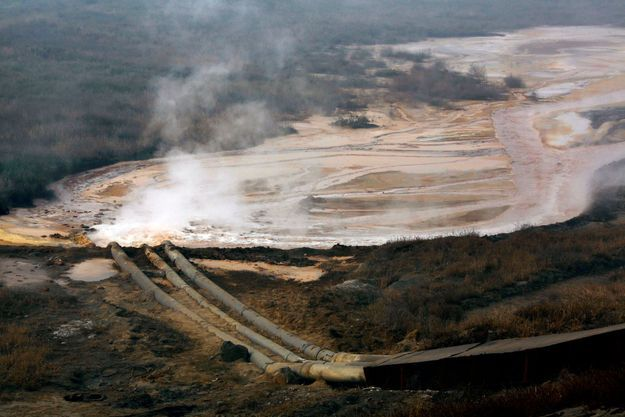
\includegraphics[scale=0.17]{Feathergraphics/lac.jpg}
    \caption{Lac de Baotou}
\end{figure}
\end{minipage}\hfill


\end{figure}

\end{block}
\begin{block}{Utilisation et destruction }
    
\begin{figure}[h!]
\begin{minipage}[b]{0.27\linewidth}
 $\nearrow$ Energie produite
\begin{figure}
    \centering
    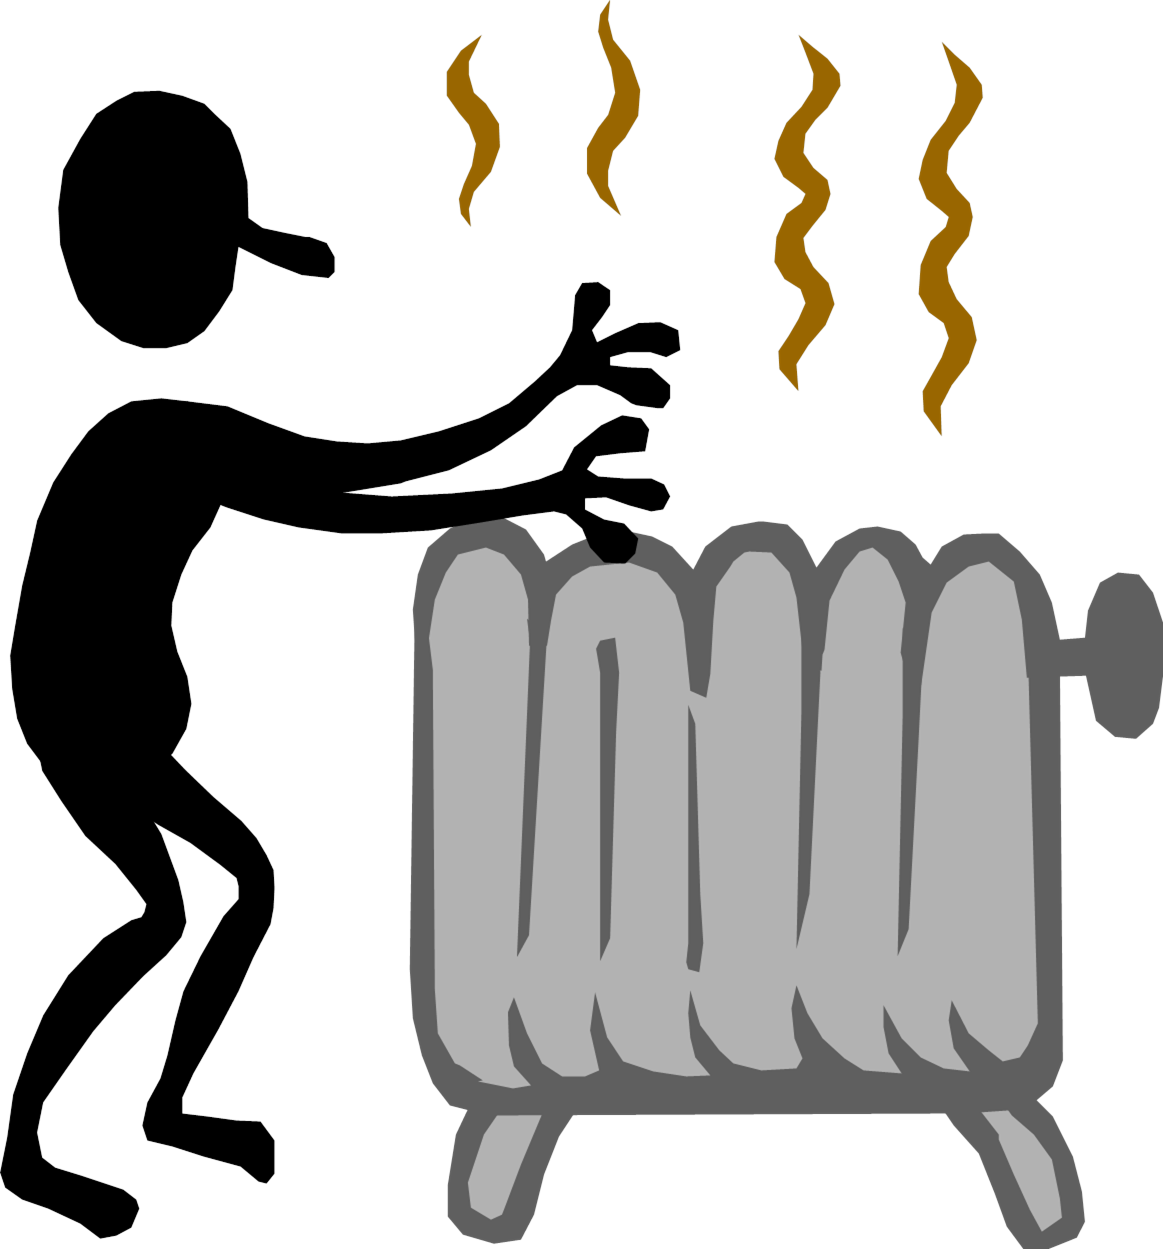
\includegraphics[scale=0.26]{Feathergraphics/rad.png}
\end{figure}
\end{minipage}\hfill
\begin{minipage}[b]{0.3\linewidth}  
4000 Data Centers

\begin{figure}
    \centering
    
\includegraphics[scale=0.03]{Feathergraphics/ville.png}
\end{figure}
\end{minipage}\hfill
\begin{minipage}[b]{0.3\linewidth}  
$5\%$ recyclés

\begin{figure}
    \centering
    
\includegraphics[scale=0.06]{Feathergraphics/poubelle.png}
\end{figure}
\end{minipage}
\end{figure}

\end{block}


\end{frame}


\section{Le Web développement}


\begin{frame}{Bonnes pratiques dans le numérique}{Conseil 1/115}

\begin{block}{Éliminer les fonctionnalités non essentielles}

\textbf{Description} : 70\% des fonctionnalités non essentielles et 45\% famais utilisées.
Niveau ergonomie, on augmente la simplicité.

\textbf{Méthodes} : maquettes, MoSCoW.


\begin{minipage}[b]{0.5\linewidth}  
\begin{figure}
    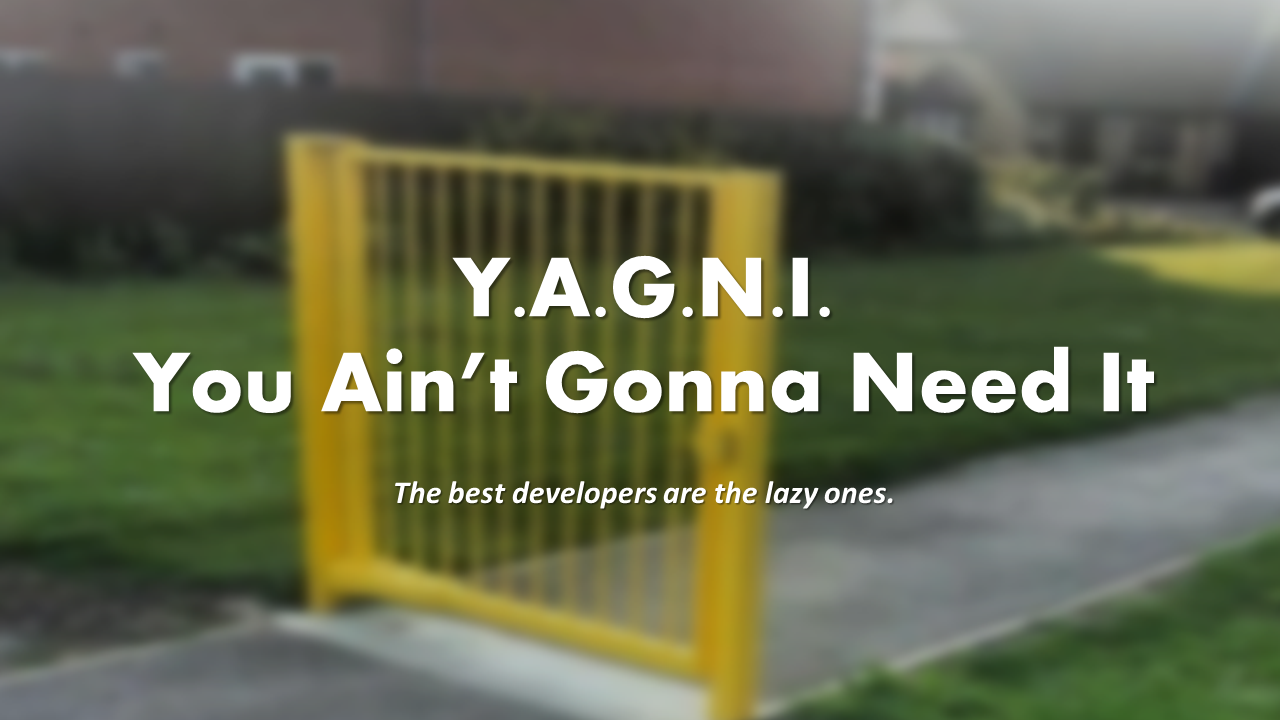
\includegraphics[scale=0.12]{chapitre2/wdd1/fig/yagni.png}
    \centering
\end{figure}
\end{minipage}\hfill
\begin{minipage}[b]{0.5\linewidth}  
\begin{figure}
    \centering
    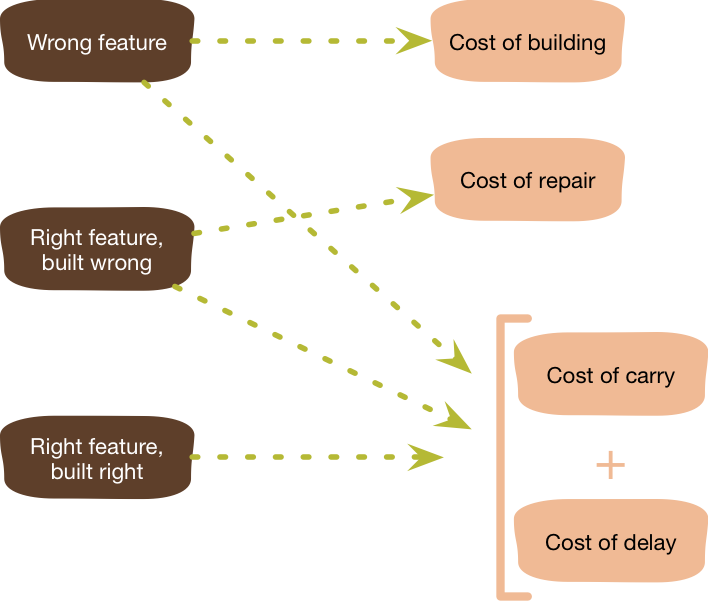
\includegraphics[scale=0.22]{chapitre2/wdd1/fig/sketch.png}
\end{figure}
\end{minipage}\hfill

\end{block}
\end{frame}

\begin{frame}{Bonnes pratiques dans le numérique}{Conseils 2-3/115}

\begin{block}{Quantifier précisément le besoin}

\textbf{Description} : Eviter la surqualité

\textbf{Exemples} : En l’absence de précision, le nombre d’items d’une liste est limité à 5 éléments.

Un nombre d’items affichés sur la page de résultats de son moteur de recherche Bing réduit jusqu’à 80\% le nombre de serveurs.

\end{block}

\begin{block}{Optimiser le parcours utilisateur}

\textbf{Description} : Diminuer le temps passé par l'utilisateur sur ses usages les plus fréquents

\textbf{Exemples} : 
\begin{enumerate}
    \item Proposer, pour un site de grande distribution, une nouvelle commande sur la base du contenu de la précédente
    \item Acheter sans inscription sur un site d'e-commerce.
    \item Copier/Coller son RIB plutôt que le télécharger puis le transférer.
    \item Mettre en avant les champs ou les filtres les plus utilisé
\end{enumerate}
\end{block}


\end{frame}

\begin{frame}{Bonnes pratiques dans le numérique}{Conseil 4/115}

\begin{block}{Préférer la saisie assistée à l'autocomplétion}

\textbf{Description} :L'autocomplétion envoie une requête au serveur à chaque caractère saisi pour récupérer les résultats correspondants (\textit{beaucoup de requêtes effectuées et de ressources dépensées}).

\textbf{Solution} :
Remplacer par la saisie assistée (guider l’utilisateur par un ensemble d’informations et d’indices)


\begin{figure}
    \centering
    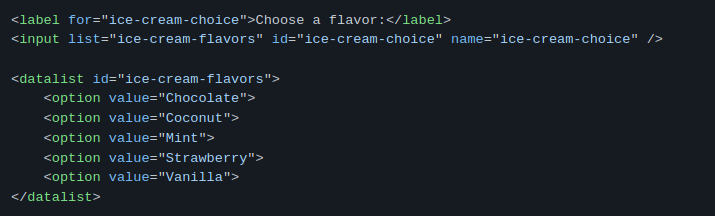
\includegraphics[scale=0.43]{chapitre2/wdd1/fig/codec.png}
\end{figure}


\end{block}

\end{frame}

\begin{frame}{Bonnes pratiques dans le numérique}{Conseils 5-6/115}

\begin{block}{Favoriser un design simple, épuré, adapté au web}

\textbf{Description} : Privilégier un design simple et épuré réalisable uniquement en HTML5 et CSS3.

\textbf{Méthode} :
 Supprimer les images de fond et ajouter un glyphe (Préférer les glyphes aux images, bonne pratique d'écoconception) avec une colorimétrie cohérente si un groupement doit avoir lieu.

\end{block}


\begin{block}{Privilégier une approche 'mobile first', à défaut un chargement adaptatif}

\textbf{Description} : Privilégier un design simple et épuré réalisable uniquement en HTML5 et CSS3.

\textbf{Exemples} :
\begin{enumerate}
    \item Côté serveur, utiliser les client hints,
    \item Côté client, media queries 
\end{enumerate}

\end{block}


\end{frame}



\begin{frame}{Bonnes pratiques dans le numérique}{Conseil 7/115}

\begin{block}{Respecter le principe de navigation rapide dans l’historique}

\textbf{Description} :
Eviter tout élément qui rendrait la page inéligible au bfcache, et/ou qui rendrait la page inutilisable après l'avoir quittée (\textit{ou éventuellement les rendre utilisables à nouveau quand la page est réutilisée, ou juste avant qu'elle soit mise en cache}).

\textbf{Solution : Eviter} 
\begin{enumerate}
    \item les actions lorsqu'on quitte la page (événements unload ou beforeunload, leur préférer pagehide si c'est vraiment nécessaire)
    \item les liens qui ouvrent de nouveaux onglets / fenêtres sans rel="noopener" ou rel="noreferrer"
    \item de laisser des connexions (IndexedDB, fetch() ou XMLHttpRequest, Web Sockets, etc.) ouvertes quand l'utilisateur quitte la page
\end{enumerate}

Utiliser les événéments \textbf{pageshow} et/ou \textbf{pagehide} pour réinitialiser les éléments, par exemple réactiver les boutons de formulaire qui se désactivent lors de la soumission ou supprimer les informations sensibles (\textit{comme les mots de passe}).
\end{block}

\end{frame}



\begin{frame}{Bonnes pratiques dans le numérique}{Conseil 8-9/115}

\begin{block}{Privilégier un traitement asynchrone}

\textbf{Description} :
Lorsque l’interaction avec l’utilisateur induit un traitement lourd et long côté serveur, proposer un traitement asynchrone.

\begin{itemize}
    \item Déclencher côté utilisateur le traitement
    \item se reconnecter quand celui-ci est terminé sans attendre sur son terminal la fin de l'exécution 
\end{itemize}


\textbf{Exemple} : Réception d’un e-mail contenant un lien. Cette approche permet de réaliser des traitements par lots (batchs), souvent plus efficients en ressources que des traitements synchrones à la volée.
\end{block}


\begin{block}{Limiter le nombre de requêtes HTTP}

\textbf{Description} :
Limiter le nombre de requêtes GET.


\textbf{Exemple} : Pour afficher des petits drapeaux pour le choix d'une langue, l'utilisation d'une spritesheet CSS permet de les regrouper dans une seule image de plus grande taille. Ce procédé réduit le nombre de requêtes HTTP.
\end{block}

\end{frame}



\begin{frame}{Bonnes pratiques dans le numérique}{Conseil 10/115}

\begin{block}{Stocker les données statiques localement}

\textbf{Description} :
Stocker localement des données structurées statiques (IndexDB, Web Storage et la mise en cache dans le Cache Storage API).

\end{block}

\begin{figure}
    \centering
    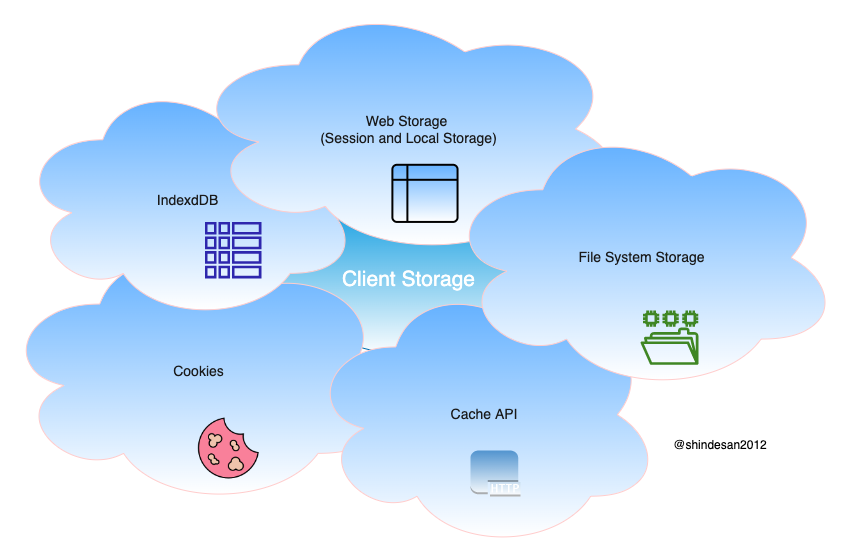
\includegraphics[scale=0.29]{chapitre2/wdd1/fig/storage.png}
\end{figure}

\end{frame}



\begin{frame}{Pause débunkage }{Fake checking : le véhicule électrique}

\begin{figure}
    \centering
    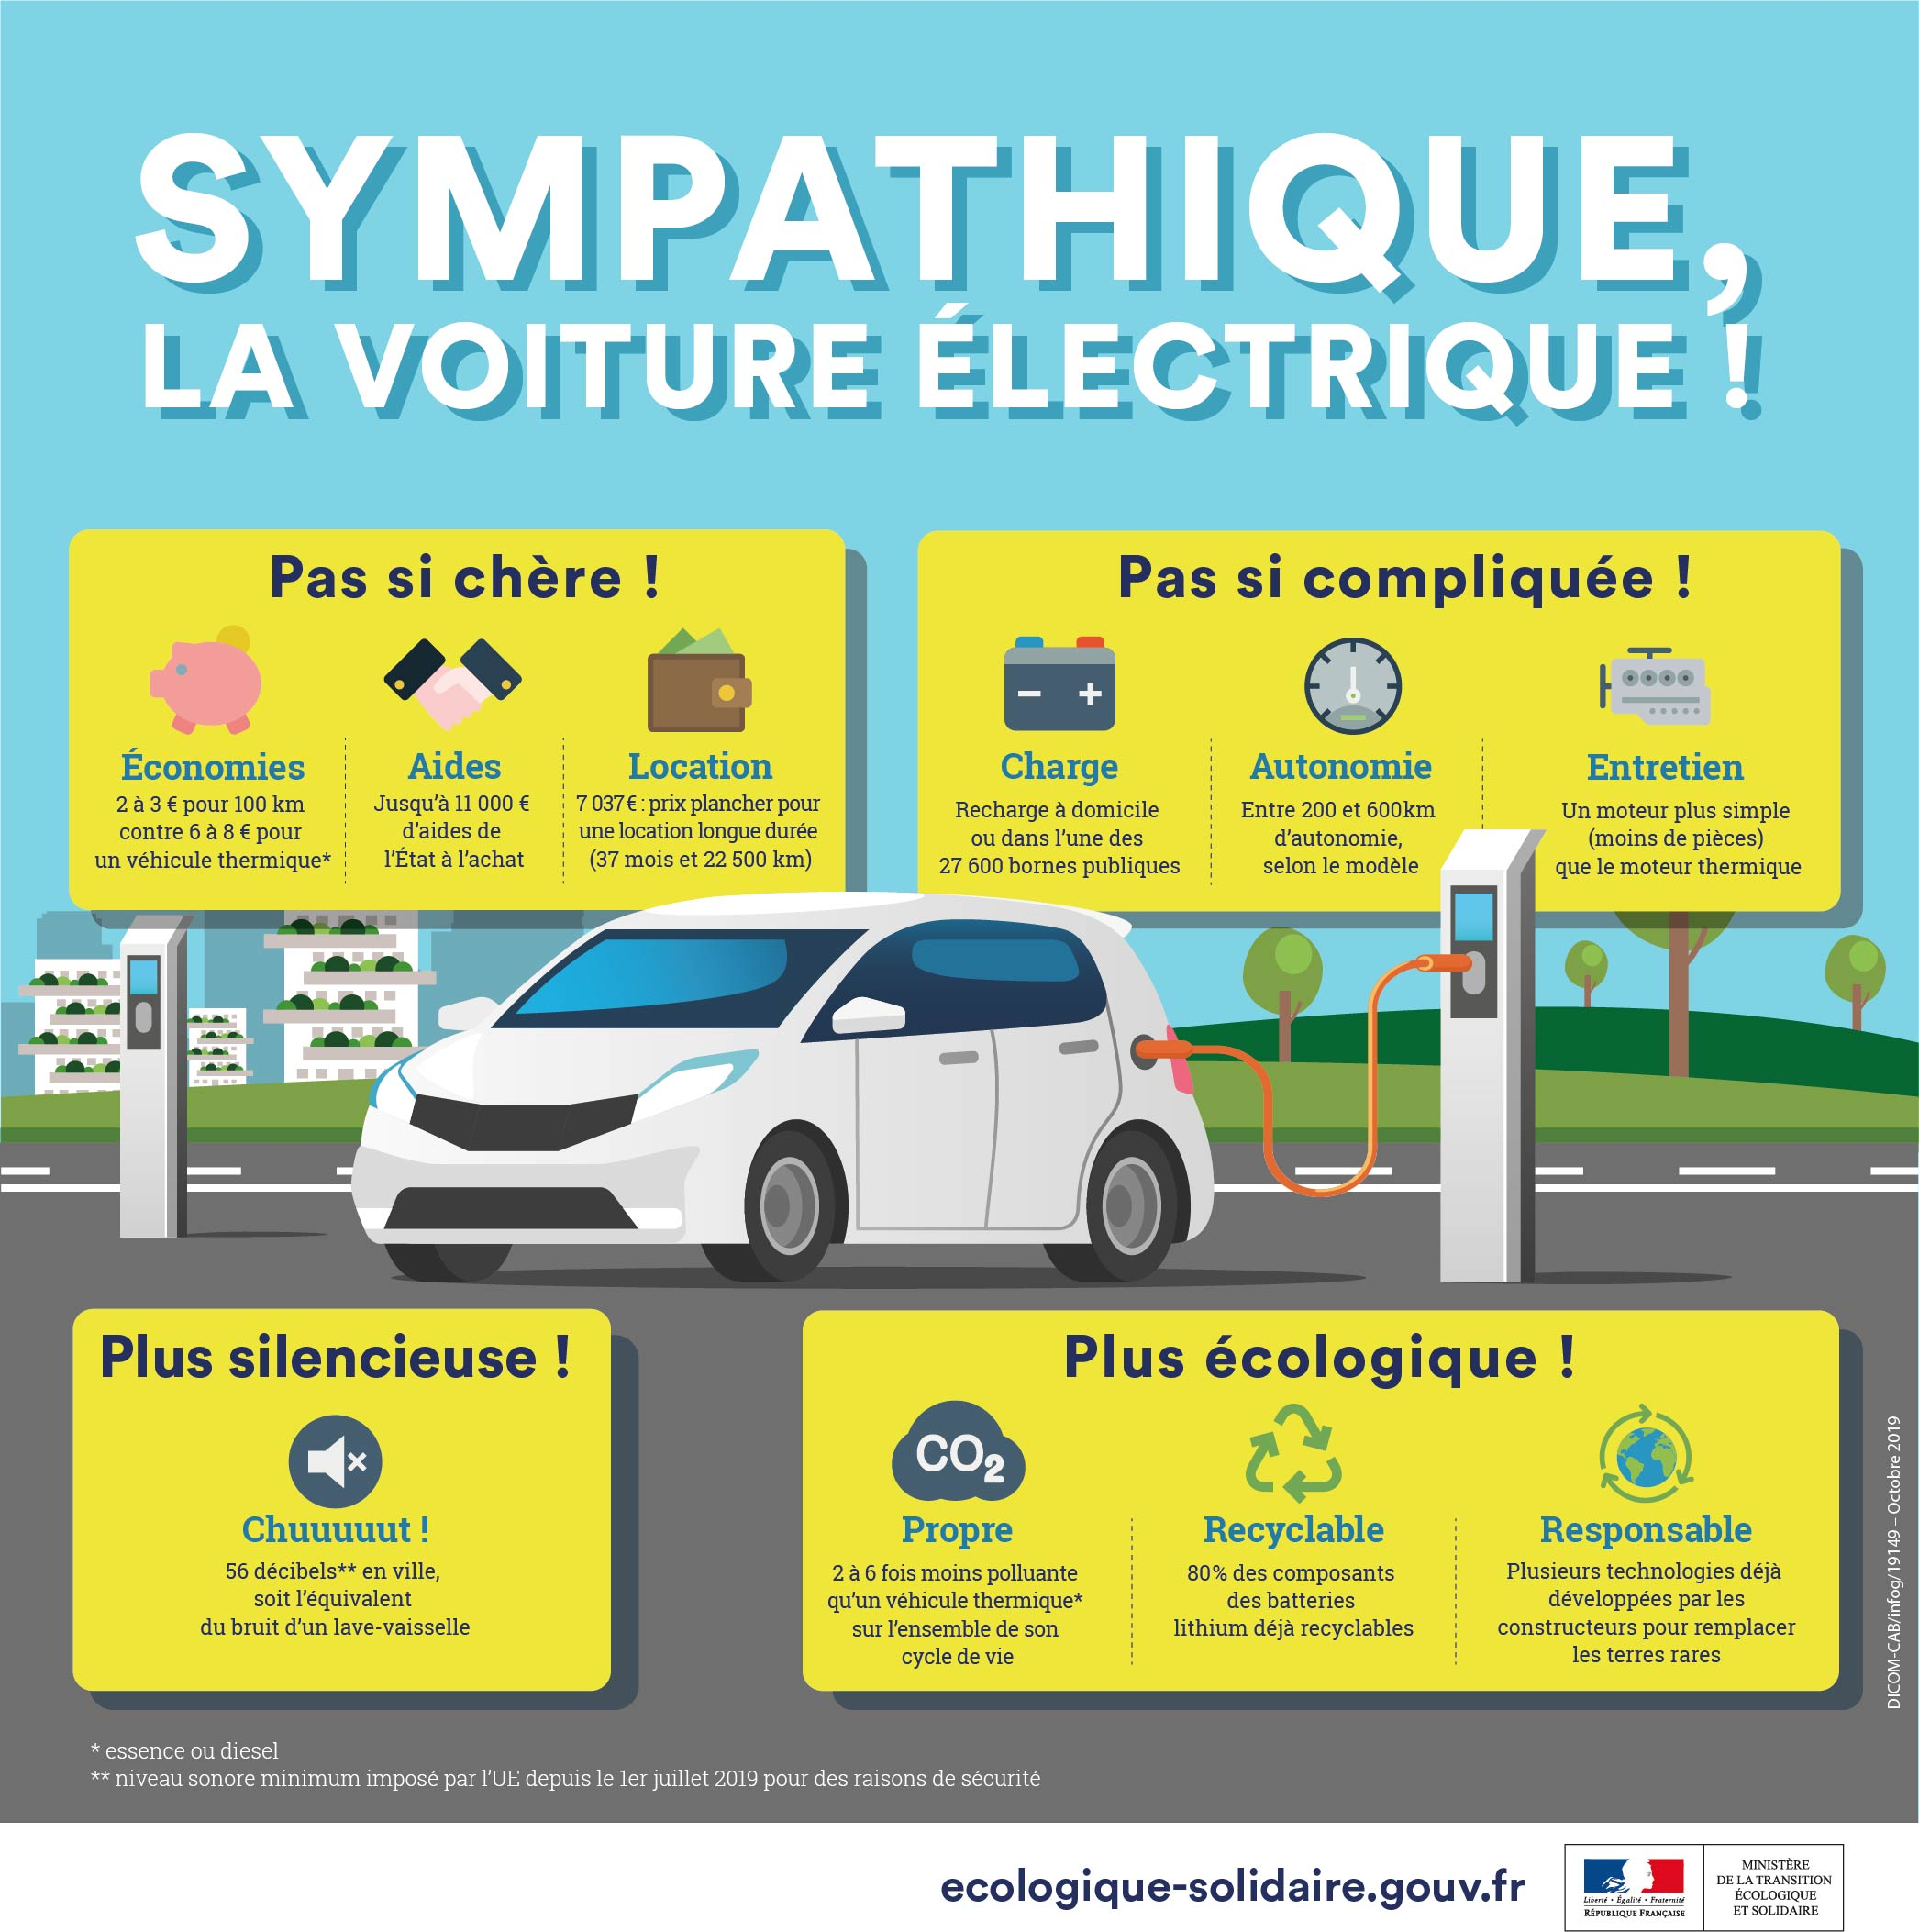
\includegraphics[scale=0.2]{chapitre2/wdd1/fig/ecovoiture.jpeg}
\end{figure}

%https://reporterre.net/Non-la-voiture-electrique-n-est-pas-ecologique#nb4

\end{frame}


\begin{frame}{Bonnes pratiques dans le numérique}{Conseils 11-14/115}

\begin{block}{Favoriser un développement sur-mesure à l'usage d'un CMS}
Les CMS utilisent des systèmes de "hook".
\end{block}

\begin{block}{Favoriser les pages statiques}
pour une landing page ou simple site vitrine de créer un site statique en HTML, CSS et JS.
\end{block}

\begin{block}{Créer une architecture applicative modulaire}
Les logiciels open source les plus efficients, comme nginX, Apache, MySQL ou PHP, reposent sur cette architecture modulaire.

Côté backend, le découpage en microservices permet d'apporter un niveau de modularité pour des services HTTP. 
\end{block}


\begin{block}{Choisir les technologies les plus adaptées}
 Sélectionner l’outil le plus économe en fonction de ses besoins et de ses contraintes métier.
\end{block}

\end{frame}


\begin{frame}{Bonnes pratiques dans le numérique}{Conseil 15/115}

\begin{block}{Utiliser certains forks applicatifs orientés "performance"}

\begin{itemize}
    \item À Redis, préférer plutôt la version optimisée KeyDB.
    \item À Drupal, préférer plutôt la version optimisée Pressflow.
\end{itemize}
\end{block}


\begin{minipage}[b]{0.4\linewidth}  
\begin{figure}
    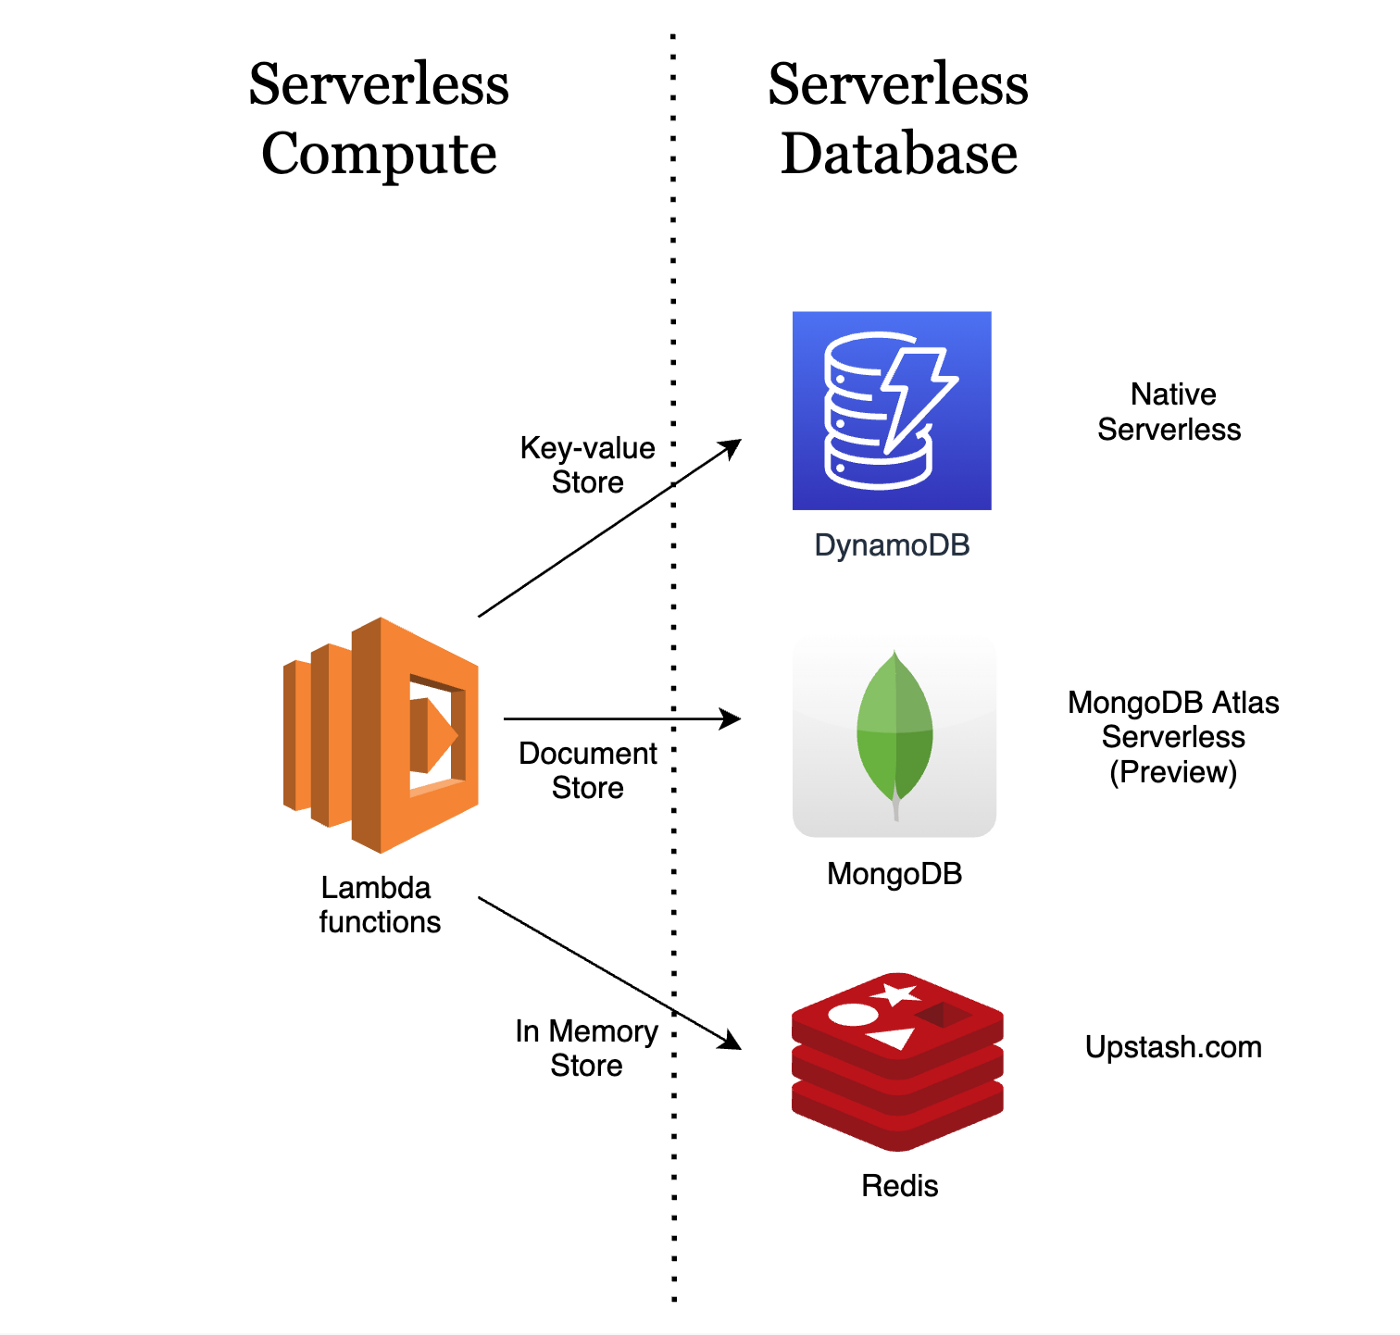
\includegraphics[scale=0.1]{chapitre2/wdd2/fig/redis.png}
    \centering
\end{figure}
\end{minipage}\hfill
\begin{minipage}[b]{0.6\linewidth}  
\begin{figure}
    \centering
    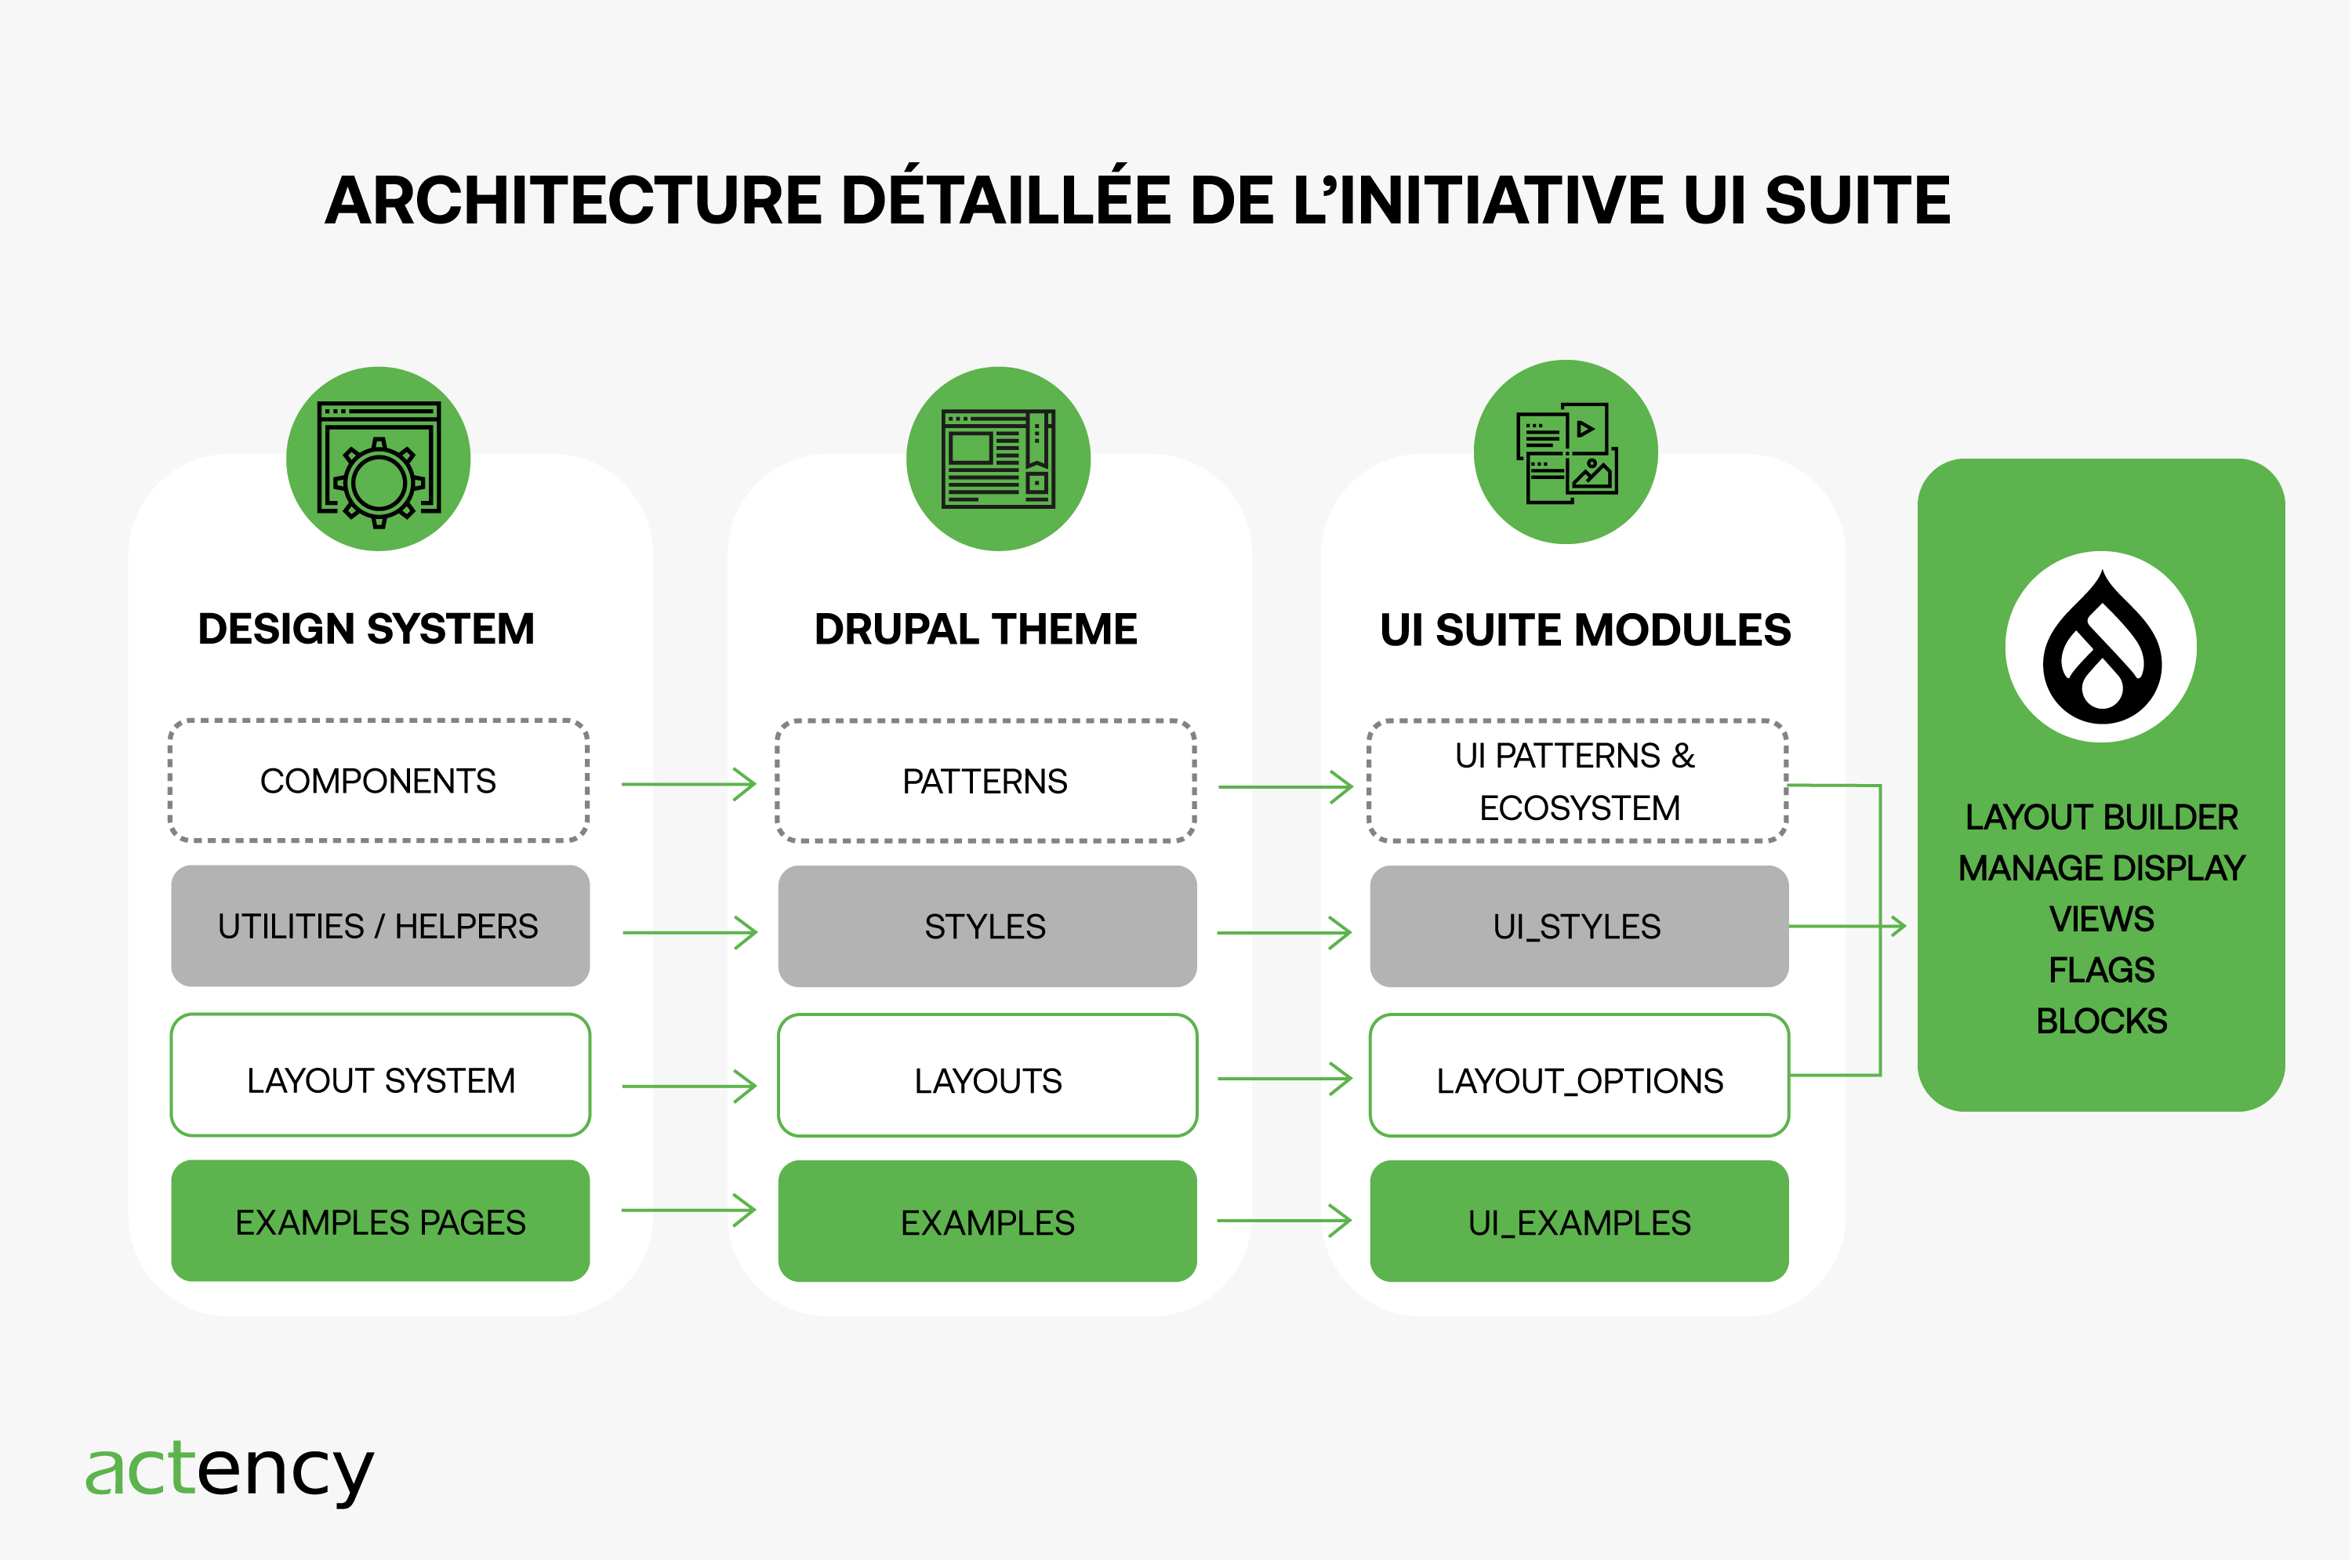
\includegraphics[scale=0.07]{chapitre2/wdd2/fig/drupal.jpg}
\end{figure}
\end{minipage}\hfill


\end{frame}

\begin{frame}{Bonnes pratiques dans le numérique}{Conseils 16-18/115}

\begin{block}{Choisir un format de données adapté}
Le type de données utilisé pour manipuler et stocker une donnée a un impact significatif sur la consommation mémoire et les cycles.
\end{block}

\begin{block}{Limiter le nombre de domaines servant les ressources}
 Regrouper toutes les ressources sur un seul domaine.
 \end{block}

\begin{block}{Remplacer les boutons officiels de partage des réseaux sociaux}
Préférer des liens HTML aux plugins JavaScript
\begin{figure}
    \centering
    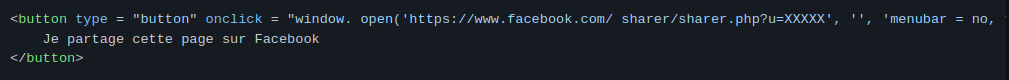
\includegraphics[scale=0.305]{chapitre2/wdd2/fig/code.png}
\end{figure}


 \end{block}
 
 
 
\end{frame}




\begin{frame}{Bonnes pratiques dans le numérique}{Conseils 19-21/115}

\begin{block}{Découper les CSS}
Employer un ensemble de CSS plutôt qu’une seule, et appeler uniquement les CSS utiles.
 \end{block}

\begin{block}{Limiter le nombre de CSS}
Limiter le nombre de CSS pour ne pas multiplier les requêtes HTTP et pour simplifier le rendu côté navigateur.

\begin{figure}
    \centering
    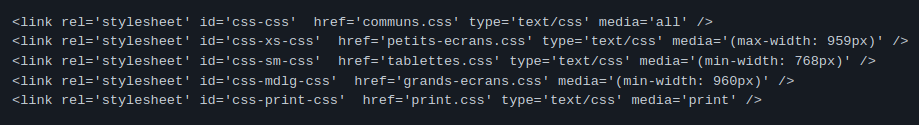
\includegraphics[scale=0.33]{chapitre2/wdd2/fig/codeL.png}
\end{figure}

 \end{block}

\begin{block}{Préférer les CSS aux images}
Utiliser les propriétés CSS3 à la place d’images. 
 \end{block}


 
\end{frame}


\begin{frame}{Pause débunkage }{Fake checking : les lampes à décharge et à led}
\begin{figure}
    \centering
    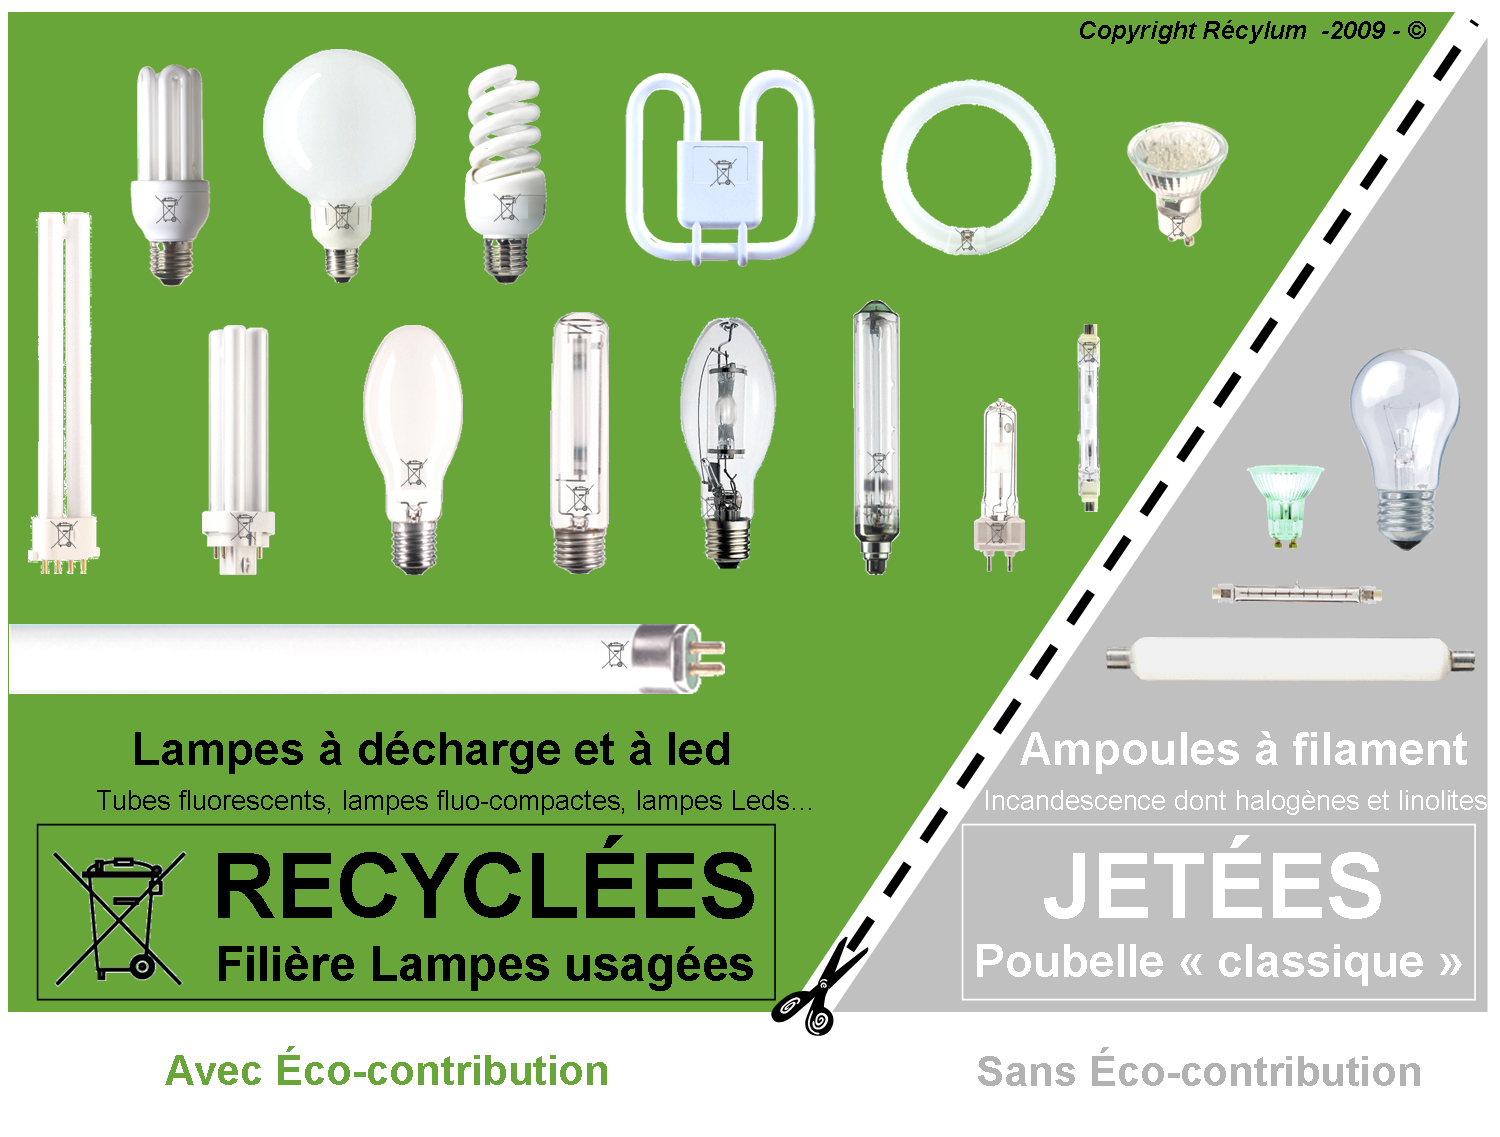
\includegraphics[scale=0.35]{chapitre2/wdd2/fig/ampoules.png}
\end{figure}

 
\end{frame}

\begin{frame}{Bonnes pratiques dans le numérique}{Conseil 22/115}

\begin{block}{Écrire des sélecteurs CSS efficaces}
Privilégier les sélecteurs basés sur des ID ou des classes. Ils seront ainsi filtrés plus rapidement, économisant des cycles CPU à la machine interprétant les règles.
 \end{block}

\begin{minipage}[b]{0.7\linewidth}
\begin{alertblock}{Ne pas écrire}
\begin{figure}
    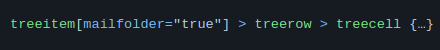
\includegraphics[scale=0.4]{chapitre2/wdd3/fig/c1.png}
    \centering
\end{figure}
 \end{alertblock}
\end{minipage}\hfill
\begin{minipage}[b]{0.3\linewidth}
\begin{exampleblock}{Mais plutôt}
\begin{figure}
    
\includegraphics[scale=0.4]{chapitre2/wdd3/fig/c2.png}
    \centering
\end{figure}
 \end{exampleblock}
\end{minipage}\hfill

\begin{minipage}[b]{0.7\linewidth}
\begin{alertblock}{Ne pas écrire}
\begin{figure}
    
\includegraphics[scale=0.5]{chapitre2/wdd3/fig/c3.png}
    \centering
\end{figure}
 \end{alertblock}
\end{minipage}\hfill
\begin{minipage}[b]{0.3\linewidth}
\begin{exampleblock}{Mais plutôt}
\begin{figure}
    
\includegraphics[scale=0.4]{chapitre2/wdd3/fig/c4.png}
    \centering
\end{figure}
 \end{exampleblock}
\end{minipage}\hfill


\end{frame}


\begin{frame}{Bonnes pratiques dans le numérique}{Conseils 24-26/115}
\begin{block}{Grouper les déclarations CSS similaires}
Lorsque plusieurs éléments du DOM (Document Object Model) ont des propriétés CSS communes, les déclarer ensemble dans la même feuille de styles. Cette méthode permet de réduire le poids de la CSS.
\end{block}

\begin{block}{Utiliser les notations CSS abrégées}
\begin{minipage}[b]{0.7\linewidth}
\begin{alertblock}{Ne pas écrire}
\begin{figure}
    
\includegraphics[scale=0.35]{chapitre2/wdd3/fig/c5.png}
    \centering
\end{figure}
 \end{alertblock}
\end{minipage}\hfill
\begin{minipage}[b]{0.3\linewidth}
\begin{exampleblock}{Mais plutôt}
\begin{figure}
    
\includegraphics[scale=0.49]{chapitre2/wdd3/fig/c6.png}
    \centering
\end{figure}
 \end{exampleblock}
\end{minipage}\hfill

\end{block}


\begin{block}{Fournir une CSS print}
La feuille de styles réduit le nombre de pages imprimées, et donc indirectement l’empreinte écologique du site web (dépouillée, police de caractères économe en encre.

\end{block}

\end{frame}


\begin{frame}{Bonnes pratiques dans le numérique}{Conseils 27-29/115}

\begin{block}{Favoriser les polices standards}
Elles sont déjà présentes sur l’ordinateur de l’utilisateur (absence de téléchargement). 
\end{block}

\begin{block}{Préférer les glyphs aux images}
\begin{itemize}
    \item Réduire la bande passante en économisant sur le poids
    \item Réduire le nombre de requêtes
    \item Réduire la complexité du DOM, notamment avec de nombreux pictogrammes SVG
\end{itemize}
\end{block}

\begin{block}{Valider les pages auprès du W3C}
Utiliser le validateur du W3C (World Wide Web Consortium) pour vérifier que les pages sont bien valides et que le code HTML est correctement formé : https://validator.w3.org
\end{block}

\end{frame}



\begin{frame}{Externaliser les CSS et JavaScript}{Conseils 30-32/115}

\begin{block}{Externaliser les CSS et JavaScript}
Veiller à ce que les codes CSS et JavaScript ne soient pas embarqués dans le code HTML de la page, à l’exception d’éventuelles variables de configuration pour les objets JavaScript.


\begin{minipage}[b]{0.5\linewidth}
\begin{alertblock}{Ne pas écrire}
\begin{figure}
    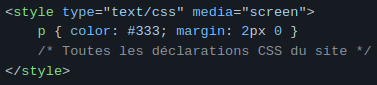
\includegraphics[scale=0.4]{chapitre2/wdd3/fig/c7.png}
    \centering
\end{figure}
 \end{alertblock}
\end{minipage}\hfill
\begin{minipage}[b]{0.45\linewidth}
\begin{exampleblock}{Mais plutôt}
\begin{figure}
    
\includegraphics[scale=0.35]{chapitre2/wdd3/fig/c8.png}
    \centering
\end{figure}
 \end{exampleblock}
\end{minipage}\hfill

\end{block}

\begin{block}{Ne pas redimensionner les images coté navigateur}
Générer les images à la taille à laquelle elles sont affichées.
\end{block}


\begin{block}{Eviter d'utiliser des images matricielles pour l'interface}
Privilégier l'approche vectorielle.
\end{block}


\end{frame}






\begin{frame}{Pause débunkage }{Le greenWashing}
\begin{figure}
    \centering
    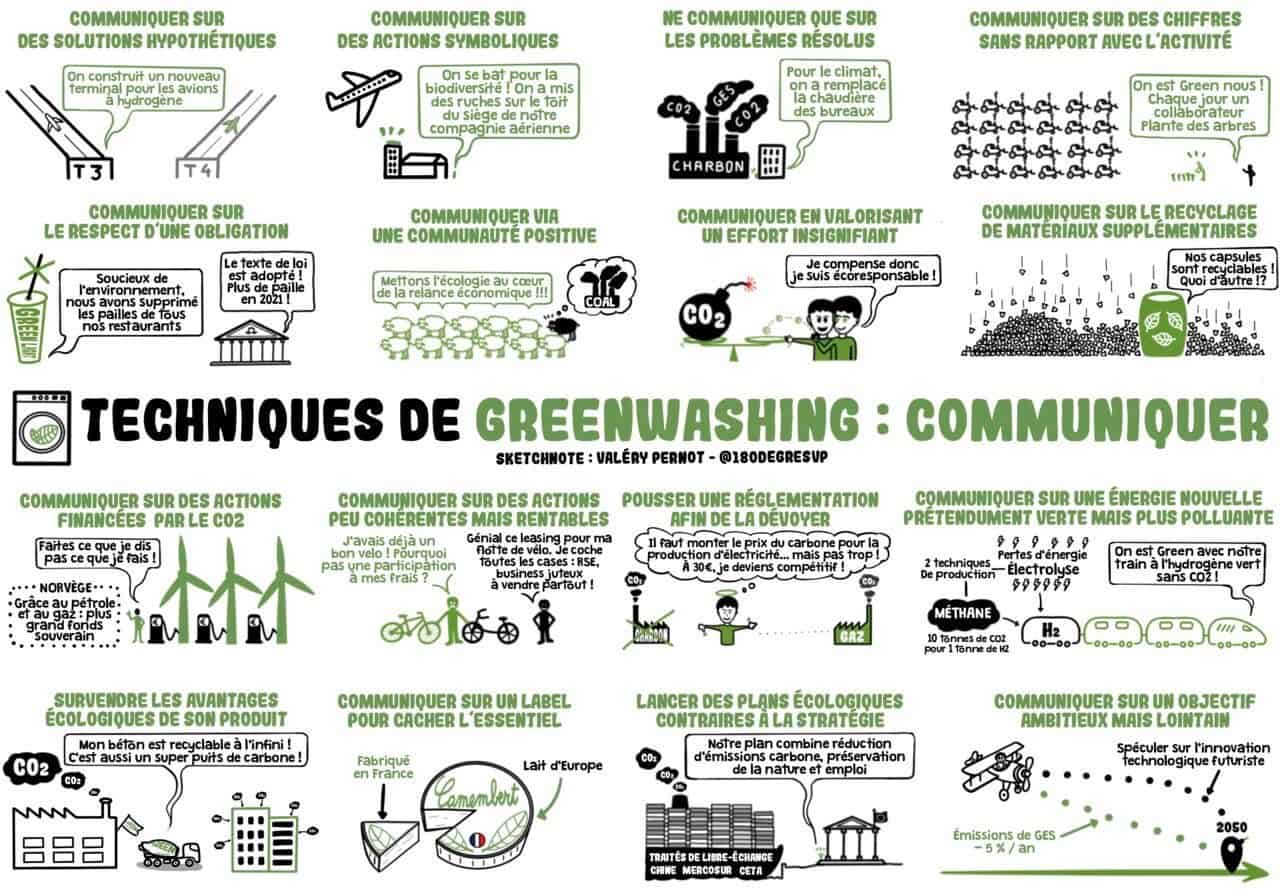
\includegraphics[scale=0.235]{chapitre2/wdd3/fig/greenwashing.jpg}
\end{figure}
\end{frame}


\begin{frame}{Bonnes pratiques dans le numérique}{Conseils 33-35/115}
\begin{block}{Optimiser les images vectorielles}

Les images SVG ont des informations de couche (layer), des commentaires, inutiles pour l’afficher. D’où l’idée de les supprimer pour réduire le poids des fichiers ( Compressor.io, SVG Cleaner, ou SVGO).
\end{block}

\begin{block}{Utiliser le chargement paresseux}
Utiliser des mini-librairies Javascript, très légères, qui s'occuperont de lazy-loader vos images ( LOZAD, Vanilla-lazyload)
\begin{figure}
    \centering
    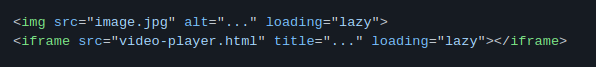
\includegraphics[scale=0.5]{chapitre2/wdd4/fig/c1.png}
\end{figure}
\end{block}

\begin{block}{Utiliser le rechargement partiel d'une zone de contenu}
Procéder à un rechargement uniquement des changements et non pas de toute la page. 
\end{block}


\end{frame}


\begin{frame}{Bonnes pratiques dans le numérique}{Conseils 36-38/115}
\begin{block}{Éviter les animations JavaScript / CSS}
Les animations JavaScript/CSS peuvent être très coûteuses en termes de cycles CPU et de consommation mémoire
\end{block}

\begin{block}{N'utilisez que les portions indispensables des librairies JavaScript et frameworks CSS}

Se passer des bibliothèques JavaScript ou n’en conserver que les portions réellement utilisées.
Utiliser un bundler (ex: Webpack) permet de faire facilement du tree shaking, soit d'éliminer du code "mort" donc non utilisé
\end{block}

\begin{block}{Ne pas faire de modification du DOM lorsqu’on le traverse}

\begin{minipage}[b]{0.35\linewidth}
Modifier le DOM (Document Object Model) est gachis en cycles CPU
\end{minipage}\hfill
\begin{minipage}[b]{0.65\linewidth}
\begin{figure}
    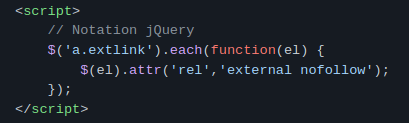
\includegraphics[scale=0.4]{chapitre2/wdd4/fig/c2.png}
\end{figure}
\end{minipage}\hfill
\end{block}
\end{frame}


\begin{frame}{Bonnes pratiques dans le numérique}{Conseils 39-40/115}
\begin{block}{Rendre les éléments du DOM invisibles lors de leur modification}

Lorsqu’un élément du DOM doit être modifié, il est plus économe de :
\begin{itemize}
    \item rendre l’élément invisible (passer la propriété display à none) (1 reflow)
    \item modifier toutes les propriétés de l’élément et rendre l’élément à nou-veau visible (1 reflow).
\end{itemize}
   \begin{figure}
    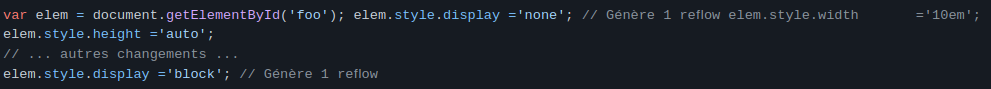
\includegraphics[scale=0.3]{chapitre2/wdd4/fig/c3.png}
\end{figure} 
\end{block}

\begin{block}{Réduire au maximum le repaint (appearence) et le reflow (layout)}

\begin{itemize}
    \item Ne pas modifier les propriétés stylistiques d’un élément
    \item Limiter les changements de propriétés de position, de dimension, de type de positionnement, de contenu
\end{itemize}

\end{block}


\end{frame}

\begin{frame}{Bonnes pratiques dans le numérique}{Conseil 41/115}
\begin{block}{Utiliser la délégation d'évènements}
La délégation d’événements permet de ne pas surcharger la mémoire du navigateur (un seul écouteur pour plusieurs éléments du DOM)

   \begin{figure}
    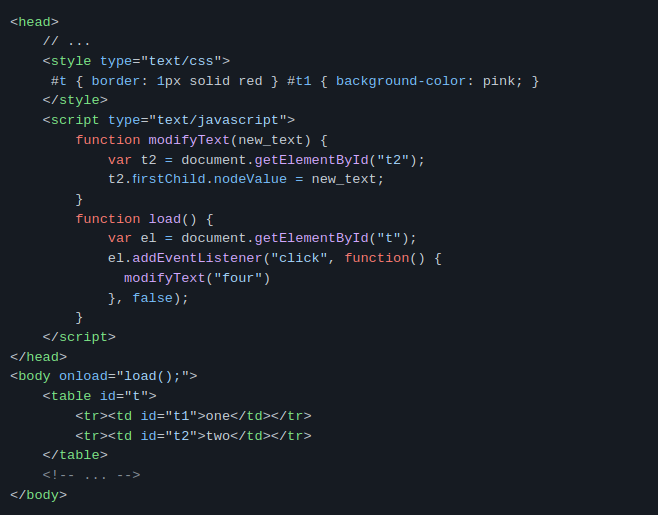
\includegraphics[scale=0.3]{chapitre2/wdd4/fig/c4.png}
\end{figure} 
\end{block}
\end{frame}




\begin{frame}{Bonnes pratiques dans le numérique}{Conseil 42-44/115}
\begin{block}{Modifier plusieurs propriétés CSS en 1 seule fois}
Ne pas modifier des propriétés une à une (plutôt modifier les classes CSS).
\end{block}
\begin{block}{Valider votre code avec un Linter}
\begin{itemize}
    \item  ESLint pour le code JavaScript
    \item Stylelint pour vs feuilles de styles
\end{itemize}
\end{block}

\begin{block}{Mettre en cache les objets souvent accédés en JavaScript}
L’accès au DOM est coûteux en cycles CPU.
\begin{figure}
    \centering
    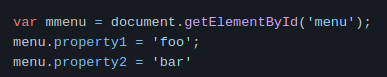
\includegraphics[scale=0.35]{chapitre2/wdd4/fig/c6.png}
\end{figure}
\begin{figure}
    \centering
    
\includegraphics[scale=0.35]{chapitre2/wdd4/fig/c7.png}
\end{figure}
\end{block}


\end{frame}


\begin{frame}{Pause débunkage }{Zones invivables}
\begin{figure}
    \centering
    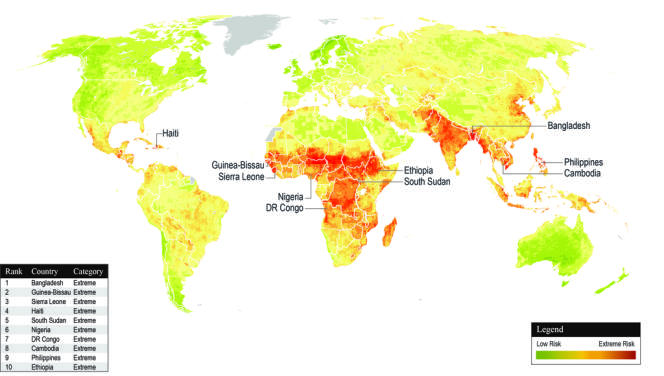
\includegraphics[scale=2]{chapitre2/wdd4/fig/climat.jpg}
\end{figure}
\end{frame}

\begin{frame}{Bonnes pratiques dans le numérique}{Conseils 45-49/115}
\begin{block}{Réduire les accès au DOM via JavaScript}
Assigner le nœud dans des variables évite de retraverser l’arbre à chaque manipulation du document.
\end{block}

\begin{block}{Utiliser tous les niveaux de cache du CMS}
Utiliser la granularité du CMS réduit les ressources consommées.
\end{block}

\begin{block}{Optimiser et générer les médias avant importation sur un CMS}
 FFmpeg, Any Video Converter, Xnview, Gimp, Inskape, PDFedit...
\end{block}

\begin{block}{Encoder les sons en dehors du site web}
Un serveur web n’est pas optimisé pour le (ré)encodage des fichiers audio.
\end{block}

\begin{block}{Mettre en cache les données calculées souvent utilisées}
Par exemple, Mettre en cache les jetons d'accès en OAuth2 et son délai d'expiration évite des appels inutiles au serveur d'autorisation.
\end{block}


\end{frame}


\begin{frame}{Bonnes pratiques dans le numérique}{Conseils 50-51/115}
\begin{block}{Supprimer tous les warning et toutes les notices}
Les warnings et notices ralentissent les serveurs d’applications tels que PHP, car ces derniers doivent retracer l’origine des erreurs et inscrire dans les différents journaux système les messages expliquant les problèmes rencontrés.
\begin{figure}
    \centering
    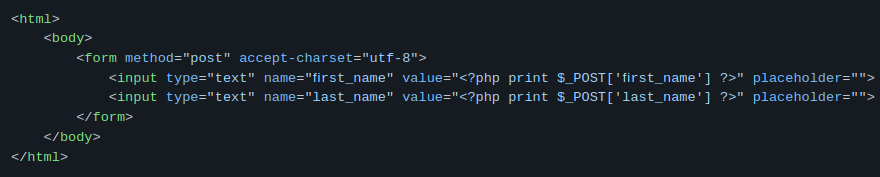
\includegraphics[scale=0.3]{chapitre2/wdd5/fig/c1.png}
\end{figure}
\end{block}

\begin{block}{Éviter d'effectuer des requêtes SQL à l’intérieur d’une boucle}
 Ces requêtes consomment inutilement des cycles CPU, de la mémoire vive et de la bande passante.
\end{block}

\end{frame}


\begin{frame}{Bonnes pratiques dans le numérique}{Conseils 52-53/115}
\begin{block}{Ne se connecter à une base de données que si nécessaire}
HikariCP est un pool de connexions JDBC solide et performant. Il est intégré dans SpringBoot.

Dans les cas où il n'y a pas de pool de connexion, réutiliser une connexion et ne pas ouvrir/fermer une nouvelle connexion à chaque requête.
\end{block}

\begin{block}{Optimiser les requêtes aux bases de données}
 Ces requêtes consomment inutilement des cycles CPU, de la mémoire vive et de la bande passante.

\end{block}

\begin{minipage}[b]{0.5\linewidth}
\begin{alertblock}{Ne pas écrire}
\begin{figure}
    
\includegraphics[scale=0.4]{chapitre2/wdd5/fig/c2.png}
    \centering
\end{figure}
 \end{alertblock}
\end{minipage}\hfill
\begin{minipage}[b]{0.5\linewidth}
\begin{exampleblock}{Mais plutôt}
\begin{figure}
    
\includegraphics[scale=0.4]{chapitre2/wdd5/fig/c3.png}
    \centering
\end{figure}
 \end{exampleblock}
\end{minipage}\hfill

\begin{figure}
    \centering
    
\includegraphics[scale=0.4]{chapitre2/wdd5/fig/c4.png}
\end{figure}
\end{frame}



\begin{frame}{Bonnes pratiques dans le numérique}{Conseils 54-56/115}
\begin{block}{Éviter le transfert d'une grande quantité de données pour réaliser un traitement}
Utiliser des  procédures stockées (SQL Server, MySQL, PostgreSQL, etc.).
\end{block}

\begin{block}{Minifier les fichiers CSS, JavaScript, HTML et SVG}

Minifier CSS, Javascript, HTML et SVG permet de supprimer les espaces inutiles, les commentaires des développeurs, les sauts de ligne, les délimiteurs de blocs et ainsi réduire leur taille.

\begin{itemize}
    \item CSS: cssnano, csso ou clean-css
    \item Javascript: Terser, UglifyJS ou Babel-minify
    \item HTML: htmlnano, HTMLMinifier
    \item SVG: SVGO, minify-xml ou équivalent
\end{itemize}

\end{block}

\begin{block}{Compresser les fichiers CSS, JavaScript, HTML et SVG}
Utiliser GZIP coté serveur, ou BROTLI côté client.
\end{block}
\end{frame}

\begin{frame}{Bonnes pratiques dans le numérique}{Conseils 57-59/115}
\begin{block}{Combiner les fichiers CSS et JavaScript}
\begin{itemize}
    \item Dans Wordpress, le plugin Autoptimize, combiner les fichiers CSS.
    \item Avec Webpack, le plugin webpack-merge-and-include-globally facilite la fusion des fichiers CSS et Javascript.
\end{itemize}
\end{block}

\begin{block}{Optimiser les images}
Outils pour réduire au minimum le poids des images :
    SQUOOSH,
    CLOUDINARY,
    ImageMagick,
    PngCrush,
    JpegTran
\end{block}

\begin{block}{Optimiser la taille des cookies}
Supprimer un cookie lorsqu’il n’est plus utile en précisant une durée d’expiration nulle ou négative.


\begin{figure}
    \centering
    
\includegraphics[scale=0.5]{chapitre2/wdd5/fig/c5.png}
\end{figure}
\end{block}
\end{frame}


\begin{frame}{Pause débunkage }{Triangle de l'inaction}
\begin{figure}
    \centering
    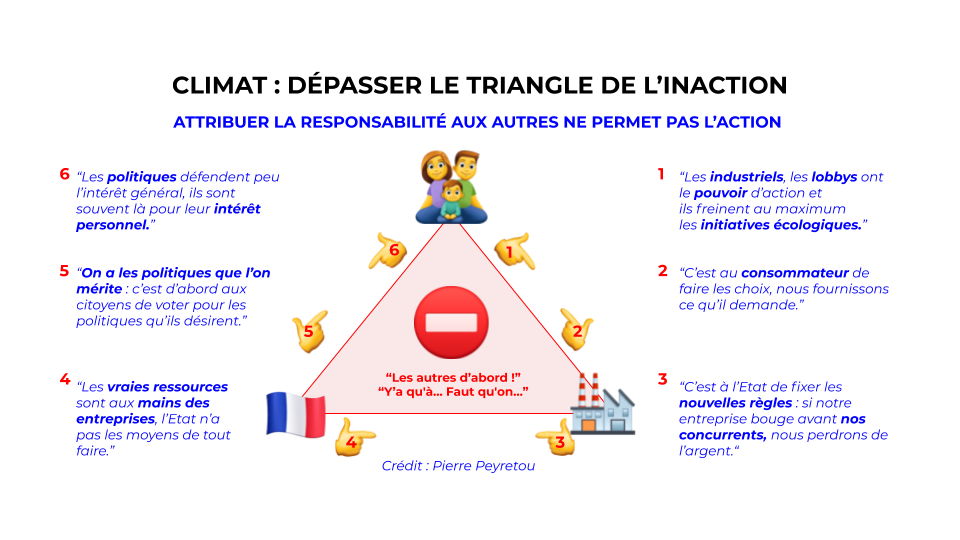
\includegraphics[scale=0.35]{Feathergraphics/[Outils Méthodo] Triangle de l'inaction.png}
\end{figure}
\end{frame}


\begin{frame}{Bonnes pratiques dans le numérique}{Conseils 60-61/115}
\begin{block}{Favoriser HSTS Preload list aux redirections 301}
Le HSTS indique à n’importe quel navigateur, via un header de réponse HTTP gardé en cache que le domaine doit exclusivement être contacté en HTTPS.
\begin{figure}
    \centering
    
\includegraphics[scale=0.45]{chapitre2/wdd6/fig/c1.png}
\end{figure}
\end{block}

\begin{block}{Mettre en place un plan de fin de vie du site}
\begin{itemize}
    \item Libérer les ressources : décommissionner le service, ses dépendances, les outils utilisés par l’équipe de développement (ex : chanel Teams).
    \item Supprimer, archiver… les données (y compris la GED et le système de suivi des bugs).
    \item Réaffecter les installations, équipements et autres ressources du projet (y compris le code source).
    \item Valoriser les compétences acquises pendant la vie du projet.
\end{itemize}
\end{block}

\end{frame}


\begin{frame}{Bonnes pratiques dans le numérique}{Conseils 62-63/115}
\begin{block}{Choisir un hébergeur écoresponsable}
\begin{enumerate}
    \item gestion des DEEE (déchets d’équipements électriques et électroniques) 
    \item efficience énergétique du data center [Power Usage Effectiveness (PUE) / Carbon Usage Effectiveness (CUE) / Water Usage Effectiveness (WUE)] 
    \item politique d’achat responsable
    \item respect de la dimension sociale
    \item alimentation aux énergies bas carbone
    \item compensation carbone
\end{enumerate}
 \textbf{Exemples :}   OVH,
    SCALEWAY,
    INFOMANIAK

\end{block}

\begin{block}{Privilégier un fournisseur d'électricité écoresponsable}
Utiliser autant que possible une électricité ayant le minimum d'impacts environnementaux lors de sa production 
\end{block}
\end{frame}


\begin{frame}{Bonnes pratiques dans le numérique}{Conseils 64-66/115}
\begin{block}{Adapter la qualité de service et le niveau de disponibilité}
La QoS et le SLA déterminés avec les utilisateurs du site web ou du service en ligne. Inutile d’héberger le service dans un centre de données très haute disponibilité (Tier IV).
\end{block}

\begin{block}{Utiliser des serveurs virtualisés}
Réduire la quantité de déchets électroniques (DEEE) et la consommation électrique.
\begin{itemize}
    \item Utiliser des outils de virtualisation tels que VMware, Xen, KVM, etc.
    \item Utiliser des outils de conteneurisation tels que Docker, Kubernetes, etc.
\end{itemize}
\end{block}

\begin{block}{Optimiser l'efficacité énergétique des serveurs} 
Privilégier des serveurs équipés d’une alimentation électrique conforme à l’écolabel 80Plus (niveaux Platinum et Titanium).

Préférer également les serveurs estampillés Energy Star.
\end{block}

\end{frame}



\begin{frame}{Bonnes pratiques dans le numérique}{Conseils 67-69/115}
\begin{block}{Installer le minimum requis sur le serveur}
Privilégier une installation "manuelle" du serveur (LAMP + CMS, par exemple) plutôt qu’une distribution avec une surcouche de type cPanel ou Plesk.

Et si une surcouche d’administration est nécessaire, préférer des solutions légères comme Webmin.
\end{block}

\begin{block}{Mettre les caches entièrement en RAM (opcode et kvs)}
Les systèmes de cache doivent être montés entièrement en mémoire vive (RAM). 
\end{block}

\begin{block}{Stocker les données dans le cloud}
Pour ne pas multiplier les domaines (conseil n° 55), le plus simple est de regrouper toutes les ressources statiques sur un seul service de stockage en ligne.
\end{block}



\end{frame}


\begin{frame}{Bonnes pratiques dans le numérique}{Conseils 70-71/115}

\begin{block}{Héberger les ressources (CSS/JS) sur un domaine sans cookie}
Les leaders du Web utilisent un domaine séparé pour servir les ressources statiques qui ne nécessitent pas de cookies. Yahoo! emploie le domaine yimg.com, YouTube le domaine ytimg.com et Amazon le domaine images-amazon.com.
\end{block}

\begin{block}{Éviter les redirections}
Les redirections dégradent le temps de réponse, tout en consommant des ressources inutilement. Il faut donc les éviter autant que possible. Ces redirections peuvent avoir lieu à différents niveaux : code HTML, code JavaScript, serveur HTTP et serveur d’applications (PHP, etc.).
\begin{figure}
    \centering
    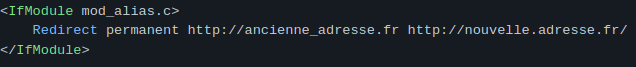
\includegraphics[scale=0.4]{chapitre2/wdd6/fig/c2.png}
\end{figure}
\end{block}

\end{frame}


\begin{frame}{Pause débunkage }{Parlons déchets}
\begin{figure}
    \centering
    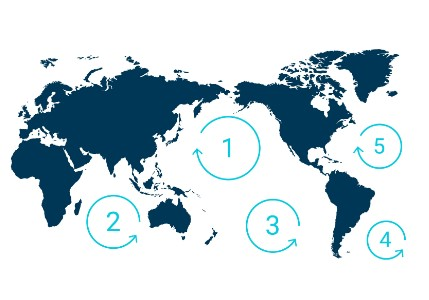
\includegraphics[scale=0.85]{chapitre2/wdd6/fig/carte.jpg}
\end{figure}
\end{frame}
\begin{frame}{Bonnes pratiques dans le numérique}{Conseils 72-74/115}
\begin{block}{Afficher des pages d'erreur statiques}
Les pages d'erreurs (40x, 50x) doivent être les plus légères possibles, et même idéalement inexistantes. 
\end{block}
\begin{block}{Utiliser un serveur asynchrone}

La plupart des serveurs web augmentent leur consommation de mémoire vive au fur et à mesure des sollicitations. Les serveurs asynchrones demeurent très stables.

Les serveurs ( Nginx, node.js ou Gwan) utilisent le minimum de ressources. 
\end{block}

\begin{block}{Utiliser un CDN (Content Delivery Network)}
Certains fichiers (bibliothèques JavaScript, les feuilles de style CSS, les images) sont gourmands en ressources réseau, car ils sont généralement nombreux et de petite taille. Utiliser les CDN, rapprochent physiquement ces fichiers des internautes, générant de ce fait un gain important de bande passante et un meilleur temps de réponse.
\end{block}


\end{frame}


\begin{frame}{Bonnes pratiques dans le numérique}{Conseils 75-76/115}
\begin{block}{Utiliser un cache HTTP}
Les reverse proxies (Varnish, Squid ou Nginx) sont optimisés pour servir du contenu (pages HTML, images, etc.) en consommant le moins de cycles CPU. 
\end{block}
\begin{block}{Ajouter des entêtes Expires ou Cache-Control}
Les en-têtes définissent la durée de conservation d'une ressource dans le cache.
\begin{figure}
    \centering
    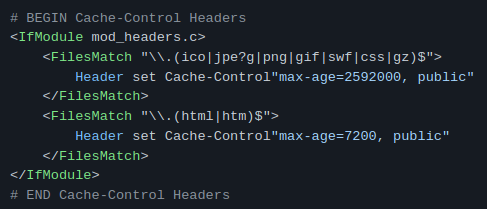
\includegraphics[scale=0.5]{chapitre2/wdd7/fig/c1.png}
\end{figure}
\end{block}
\end{frame}




\begin{frame}{Bonnes pratiques dans le numérique}{Conseils 76-78/115}
\begin{block}{Mettre en cache les réponses Ajax}
Les réponses Ajax qui seront inchangées dans un futur proche ne doivent pas être redemandées au serveur. Par conséquent, les mettre en cache économise la bande passante.
\end{block}

\begin{block}{Réduire au nécessaire les logs des serveurs}
Les logs des serveurs (web, applicatif, base de données) pouvant devenir très volumineux, il est recommandé de les configurer dans leur ensemble.
\begin{figure}
    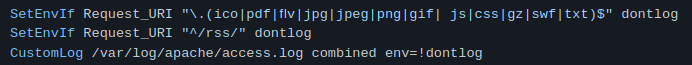
\includegraphics[scale=0.4]{chapitre2/wdd7/fig/c2.png}
\end{figure}
\end{block}

\begin{block}{Désactiver le DNS lookup d’Apache}
Quand un serveur web reçoit une requête HTTP, il enregistre cette information dans un log, en traduisant l’adresse IP de l’internaute en nom de domaine. 
\end{block}

\end{frame}


\begin{frame}{Bonnes pratiques dans le numérique}{Conseils 79-82/115}
\begin{block}{Apache Vhost : désactiver le AllowOverride}
 Le serveur HTTP Apache remonter toute la hiérarchie des répertoires pour y trouver un fichier .htaccess contenant des règles de surcharge. 
\end{block}
\begin{block}{Désactiver les logs binaires}
 Les logs binaires du serveur MySQL ou MariaDB peuvent être volumineux.
\end{block}

\begin{minipage}[b]{0.5\linewidth}
\begin{figure}
    
\includegraphics[scale=0.4]{chapitre2/wdd7/fig/c4.png}
    \centering
\end{figure}
\end{minipage}\hfill
\begin{minipage}[b]{0.5\linewidth}
\begin{figure}
    
\includegraphics[scale=0.4]{chapitre2/wdd7/fig/c3.png}
    \centering
\end{figure}
\end{minipage}\hfill


\begin{block}{Compresser les documents}
Un document pèse moins une fois compressé.
\end{block}

\begin{block}{Optimiser les PDF}
PDF adapté (taux d’échantillonnage et de compression des images, polices incorporées, résolution).
\end{block}

\end{frame}


\begin{frame}{Bonnes pratiques dans le numérique}{Conseils 83-85/115}
\begin{block}{Limiter les e-mails lourds et redondants}
Raisonner l'envoi d'e-mail automatiques (newsletters, gestion client, suivi de commande) en limitant leur nombre, les pièces jointes et le nombre de destinataires.
\end{block}

\begin{block}{Adapter les sons aux contextes d'écoute}
Privilégier 3 formats couvrant les 3 grandes plates-formes (Windows, Mac OS X et Linux) :
\begin{itemize}
    \item MP3 (MPEG-1 Audio Layer 3) ;
    \item  AAC (Advanced Audio Coding) ;
    \item Vorbis.
\end{itemize}
\end{block}

\begin{block}{Adapter les textes au web}
Ecrire des textes courts à l’aide d’un style direct.
\end{block}

\end{frame}

\begin{frame}{Bonnes pratiques dans le numérique}{Conseils 86-88/115}
\begin{block}{Adapter les vidéos aux contextes de visualisation}
Prévoir plusieurs formats (taille, frame rate, compression audio, etc.) selon le contexte de lecture des vidéos (ordinateur de bureau, tablette Wi-Fi, smartphone EDGE. ).
\end{block}

\begin{block}{N'utiliser que des fichiers double opt-in}
Le double opt-in est une pratique marketing consistant à demander le consentement du prospect, généralement par accord électronique en cochant une case, puis à faire valider ce consentement par l’envoi d’un e-mail de confirmation à l’adresse indiquée. 
\end{block}

\begin{block}{Limiter les outils d'analytics et les données collectées}
Les outils utilisés pour suivre les actions des utilisateurs utilisent souvent beaucoup de ressources coté client : requêtes nombreuses, fichiers javascripts supplémentaires chargés, utilisation de plusieurs domaines additionnels, envoi de cookie, ...
\end{block}

\end{frame}



\begin{frame}{Pause débunkage }{Parlons applications et dopamine}
\begin{figure}
    \centering
    
\includegraphics[scale=0.5]{chapitre2/wdd7/fig/dopa.png}
\end{figure}
\end{frame}




\begin{frame}{Bonnes pratiques dans le numérique}{Conseils 89-90/115}
\begin{block}{Limiter l'utilisation des GIFs animés}
Le gif animé, format image animée datant de 1995, est plus lourd et plus lent que d'autres formats tels que les formats vidéo webm ou le mp4. Le webp animé est moindre dans son gain de poids et est actuellement peu supporté par les navigateurs.
\begin{figure}
    \centering
    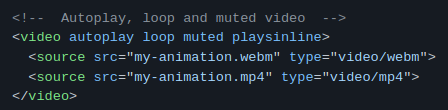
\includegraphics[scale=0.4]{chapitre2/wdd8/fig/c1.png}
\end{figure}
\end{block}

\begin{block}{Éviter la lecture/chargement automatique des vidéos/sons}L'activation automatique des vidéos et des sons au chargement des pages web implique une utilisation de ressources sur chaque tiers.

\begin{figure}
    \centering
    
\includegraphics[scale=0.4]{chapitre2/wdd8/fig/c2.png}
    
\includegraphics[scale=0.4]{chapitre2/wdd8/fig/c3.png}
\end{figure}
\end{block}
\end{frame}


\begin{frame}{Bonnes pratiques dans le numérique}{Conseils 91-93/115}
\begin{block}{Utiliser les compartiments CSS}
Le CSS Containment indique qu'un nœud et son contenu sont, autant que possible, indépendants du reste de l'arborescence de la page.
\end{block}

\begin{block}{Fournir une alternative textuelle aux contenus multimédias}

Le texte utilise beaucoup moins de bande passante que des formats multimédias comme l'audio ou la vidéo. 

\end{block}
\begin{block}{Privilégier HTTP/2 à HTTP/1}
Le protocole HTTP/2 a troqué la représentation textuelle des requêtes et réponses pour une représentation binaire avec un mécanisme de compression des entêtes HTTP (HPACK). Il permet aussi le multiplexage des échanges, permettant de n'utiliser qu'une seule connexion TCP (et donc un seul handshake TLS) avec le serveur, et ainsi tirer le meilleur avantage de HPACK.
\end{block}
\end{frame}



\begin{frame}{Bonnes pratiques dans le numérique}{Conseils 94-96/115}
\begin{block}{Économiser de la bande passante grace à un ServiceWorker}
La plupart des pages partagent une structure commune encadrant le "contenu utile". 
\end{block}

\begin{block}{Mettre en place un sitemap efficient}
Le sitemap facilite l'indexation des pages et des contenus d'un site web par les moteurs de recherche. Un sitemap non mis à jour peut contenir des urls qui n'ont plus raison d'y être car elles font référence à des pages ou des contenus peu visités et peu utiles. 
\end{block}

\begin{block}{Assurer la compatibilité avec les plus anciens appareils et logiciels du parc}
S'assurer de la compatibilité du site avec les plus anciens matériels et logiciels que les utilisateurs peuvent possèder. Les pages doivent être utilisables sur les configurations les plus contraignantes : pas de mises en page cassées, de boutons inactifs ou autre problème empêchant la lecture.
\end{block}

\end{frame}


\begin{frame}{Bonnes pratiques dans le numérique}{Conseils 97-98/115}
\begin{block}{Réduire le volume de données stockées au strict nécessaire}
Réduire le volume de données stockées par l'optimisation et la suppression.
\end{block}

\begin{block}{Utiliser une politique d'expiration/suppression des données}
 Il est obligatoire d'après le RGPD par la CNIL.
\begin{figure}
    \includegraphics[scale=0.35]{chapitre2/wdd8/fig/c4.png}
\end{figure}

\end{block}


\end{frame}


\begin{frame}{Bonnes pratiques dans le numérique}{Conseils 99-101/115}
\begin{block}{Limiter le recours aux canvas}
L'élément HTML canvas est initialement conçu pour dessiner des graphiques, réaliser des jeux ou générer des images à la volée via des API JavaScript.
\end{block}

\begin{block}{S'assurer que les parcours utilisateurs permettent de réaliser leur action prévue}
Des services web permettent de réaliser sans se déplacer des démarches administratives, des ouvertures de contrats, des déclarations de sinistres etc.
\end{block}

\begin{block}{Avoir un titre de page et une metadescription pertinents avec le contenu de la page}
Un titre de page <h1>, ainsi que son équivalent <title>, adjoints à une balise <meta name="description"> pertinente doivent être parfaitement en accord avec le contenu de la page associée. 
\end{block}

\end{frame}




\begin{frame}{Bonnes pratiques dans le numérique}{Conseils 99-101/115}
\begin{block}{Limiter le recours aux canvas}
L'élément HTML canvas est initialement conçu pour dessiner des graphiques, réaliser des jeux ou générer des images à la volée via des API JavaScript.
\end{block}

\begin{block}{S'assurer que les parcours utilisateurs permettent de réaliser leur action prévue}
Des services web permettent de réaliser sans se déplacer des démarches administratives, des ouvertures de contrats, des déclarations de sinistres etc.
\end{block}

\begin{block}{Avoir un titre de page et une metadescription pertinents avec le contenu de la page}
Un titre de page <h1>, ainsi que son équivalent <title>, adjoints à une balise <meta name="description"> pertinente doivent être parfaitement en accord avec le contenu de la page associée. 
\end{block}

\end{frame}


\begin{frame}{Pause débunkage }{Nudge}
\begin{figure}
    \centering
    \includegraphics[scale=1]{chapitre2/wdd8/fig/Nudge.jpg}
\end{figure}
\end{frame}


\begin{frame}{Bonnes pratiques dans le numérique}{Conseils 102-105/115}
\begin{block}{Utiliser la version la plus récente du langage}
Les langages côté serveurs (PHP, Ruby, Java) sont régulièrement améliorés par les différentes communautés (performances, de gestion mémoire, de stabilité et comble des failles de sécurité).
\end{block}

\begin{block}{Ne charger des données/du code que lorsqu'elles sont/il est nécessaire}
Les préchargements gaspillent des ressources.
\end{block}


\begin{block}{Éliminer les fonctionnalités non utilisées}

Piloter/supprimer certains usages de fonctionnalités.

\end{block}


\begin{block}{PWA > application mobile native similaire au site web}
 Définir les supports nécessaires en fonction des utilisateurs. Un site internet responsive peut-être tout à fait suffisant et satisfaisant.
\end{block}

\end{frame}

\begin{frame}{Bonnes pratiques dans le numérique}{Conseils 106-109/115}
\begin{block}{Éviter les temps de blocages par des traitements javascript trop longs}
 Découper vos JavaScript en petites tâches exécutées au moment requis et non pas avant.
\end{block}

\begin{block}{Mettre en place une architecture élastique}
 Modifier dynamiquement et automatiquement la taille de l'infrastructure en fonction de la charge. 
\end{block}


\begin{block}{Éliminer les fonctionnalités non utilisées}

Piloter/supprimer certains usages de fonctionnalités.

\end{block}


\begin{block}{Limiter le nombre d'appels aux API HTTP}
Fixer des quotas afin d'inciter les utilisateurs à définir une stratégie de mise en cache des réponses et éviter des appels systématiques. 
\end{block}

\end{frame}



\begin{frame}{Bonnes pratiques dans le numérique}{Conseils 110-114/115}
\begin{block}{Limiter le recours aux carrousels}
Limiter au maximum l'utilisation des carrousels en privilégiant du contenu statique mis à jour régulièrement. 
\end{block}

\begin{block}{Avoir une stratégie de fin de vie des contenus}
Supprimer les contenus non utilisés. 
\end{block}


\begin{block}{Mettre en place un "Circuit breaker"}
Un "circuit breaker" casse le traitement d'une requête à travers plusieurs services dans le cas où un des services ne répond pas.

\end{block}


\begin{block}{Favoriser le "Request collapsing"}
Limiter le nombre d’appels distants en regroupant plusieurs requêtes pour n’en faire qu’une seule.
\end{block}

\end{frame}


\begin{frame}{Pause débunkage }{L'agriculture}
%https://www.contrepoints.org/2022/05/05/380845-comment-lagro-ecologie-va-affamer-des-millions-de-personnes

\begin{figure}
    \centering
    \includegraphics[scale=0.5]{chapitre2/wdd9/fig/agri.jpg}
\end{figure}
\end{frame}


\begin{frame}{Bonnes pratiques dans le numérique}{Conseil 115/115}
\begin{block}{Ne pas afficher les documents à l'intérieur des pages}
Pour être affiché, un fichier de traitement de texte devra, par exemple, appeler un logiciel adapté. Or si ce logiciel n'est pas installé sur le poste de l'utilisateur, le fichier ne pourra pas être lu sans un développement spécifique coûteux. Il est donc préférable d'insérer un lien de téléchargement du document à l'intérieur de votre page afin que seuls les utilisateurs concernés le téléchargent.
\end{block}

\end{frame}

\begin{frame}{Bonnes pratiques dans le numérique}{Comment faire un site éco-responsable ? Côté serveur}
%-------------------------------------------------------
\begin{block}{Quelques PUE, proximité}

\begin{minipage}[b]{0.6\linewidth}

\begin{itemize}
\item Infomaniak
\item Planethoster
\item Ikoula
\item Varnish
\item Web Engine
\item Hostpapa 
\item Ionos (1\&1)
    %\item Un fond sombre demande moins de ressources qu’un fond blanc. 
    %\item Privilégier les animations 2D aux 3D. Elles sont moins gourmandes en ressources.
    %\item Les vidéos utilisent beaucoup de bandes passantes sur les serveurs. Il vaut mieux utiliser des visuels légers.
    %\item Pour avoir une empreinte carbone faible, un site web éco-responsable doit être composé de texte et d’illustrations.
    %\item Dans le choix de format pour les photos, il est préférable d’opter pour le WebP, WebM ou SVG. JPG, Png et Mp4 sont à utiliser en dernier recours.
\end{itemize}
Regarder si compression Gzip accessible

\end{minipage}\hfill
\begin{minipage}[b]{0.35\linewidth}  
\begin{figure}
    \centering
    \includegraphics[scale=0.05]{Feathergraphics/datacenter.jpg}
\end{figure}
\end{minipage}\hfill
\end{block}
\begin{block}{Et comment connaitre con empreinte carbone ?}

\url{https://www.websitecarbon.com/}
\end{block}

\end{frame}
%
\begin{frame}{Bonnes pratiques dans le numérique}{Comment faire un site éco-responsable ? Côté client}
%-------------------------------------------------------
\begin{block}{UX, conseils de développement web}

\begin{minipage}[b]{0.45\linewidth}

\begin{itemize}
\item un site rapide 
\begin{itemize}
    \item SEO 
    \item PWA
    \item CMS
    \item CDN
\end{itemize}
\item un site inclusif
\begin{itemize}
    \item statiques
\end{itemize}
\item un site mobile 
\begin{itemize}
    \item AMP
\end{itemize}
\end{itemize}
\end{minipage}\hfill
\begin{minipage}[b]{0.55\linewidth}  
\begin{itemize}
\item un site ergonomique 
\begin{itemize}
    \item peu de frictions dans l'UX
    \item choix intelligent des images, vidéos
    \item bloquer les bots
    \item dernière version de php
\end{itemize}
\item un site simple 
\begin{itemize}
    \item texte
    \item police de caractère
    \item font sombre
\end{itemize}
\end{itemize}

\end{minipage}\hfill
\end{block}
    
\end{frame}

\section{Quelques conseils de bonnes pratiques}

%https://github.com/cnumr/best-practices/blob/main/chapters/BP_095_fr.md

\begin{frame}{Quelle est l'empreinte carbone ? }
%-------------------------------------------------------

\begin{block}{Tests sur différents sites}

\begin{minipage}[b]{0.5\linewidth}
\begin{itemize}
\item \href{https://www.websitecarbon.com/}{Web Carbon Calculator}
\item \href{https://www.websitecarbon.com/website/univ-fcomte-fr/}{UFR-ST}
\item \href{https://www.websitecarbon.com/website/mcdonalds-fr/}{McDonald}
\item \href{https://www.websitecarbon.com/website/biocoop-fr-gclidcj0kcqia-eembhcparisaazfxzcs3nwxf-5givohpm1_79vyloxmb8cff4vai8q_0ymev_jfyixcyoaaav51ealw_wcb/}{Biocoop}
\item \href{https://www.websitecarbon.com/website/youtube-com/}{Youtube}
\item \href{https://www.websitecarbon.com/website/9gag-com/}{9gag}
\item \href{https://www.websitecarbon.com/website/tiktok-com-fr/}{tiktok}
\item \href{https://www.websitecarbon.com/website/wikipedia-org/}{wikipédia}
\item \href{https://www.websitecarbon.com/website/amazon-fr/}{amazon}

\item \href{https://www.red-inc.com/}{Optimisation technologique}

\end{itemize}

\end{minipage}\hfill
\begin{minipage}[b]{0.5\linewidth}  
\begin{figure}
    \centering
    \includegraphics[scale=0.17]{Feathergraphics/int.png}
\end{figure}
\end{minipage}\hfill
\end{block}

\end{frame}



\section{Conclusion}


\begin{frame}{Conclusion}{ Responsabiliser plutôt que culpabiliser}
%-------------------------------------------------------

\begin{figure}
    \centering
    \includegraphics[scale=0.35]{Feathergraphics/[Outils Méthodo] Triangle de l'inaction.png}
\end{figure}

\end{frame}


\begin{frame}[allowframebreaks]
        \frametitle{References}
        \bibliographystyle{amsalpha}
        \bibliography{biblio.bib}
\end{frame}

\begin{frame}{Merci pour votre attention !}
    		\begin{center}
	\includegraphics[scale=0.4]{EVE-icon.png}
	
	Des Questions ?
	\end{center}

\end{frame}




\begin{frame}{Impact du numérique}{des exemples d'utilisation polluante}

\begin{figure}[h!]

\begin{minipage}[b]{0.6\linewidth}
    \begin{figure}
        \centering
        \includegraphics[scale=0.2]{Feathergraphics/mail.png}
    \end{figure}
\end{minipage}\hfill
\begin{minipage}[b]{0.3\linewidth}  
\begin{figure}
    \centering
    \includegraphics[scale=0.17]{Feathergraphics/datacenter.png}
\end{figure}
\end{minipage}\hfill


\end{figure}


\end{frame}



\end{document}
